\documentclass[10pt]{article}
\usepackage{mathptmx, amsmath}
\usepackage[margin=1in]{geometry}
\usepackage{rotating, graphicx}
\usepackage[table]{xcolor}
\usepackage{natbib}
\usepackage{url}
\usepackage{threeparttable}
\usepackage{multirow}

\usepackage{array}
\newcolumntype{L}[1]{>{\raggedright\let\newline\\\arraybackslash\hspace{0pt}}p{#1}}

\title{Commercial Travel Module Version 3.0 Update}
\author{Rick Donnelly}
\date{\today}

\begin{document}
\raggedbottom
\newcommand{\gray}{\rowcolor[gray]{.95}}
\setlength\extrarowheight{2pt}
\fontsize{11.75}{14.25}\rm
\setlength{\bibsep}{0pt}
\bibliographystyle{agsm}

% Ignore glossary entries in the document
\newcommand{\gls}{}

\maketitle

\begin{abstract}
\normalsize 
\noindent The commercial travel (CT) module of the Oregon Statewide Integrated Model Version 2 (SWIM2) system simulates local and long-distance travel made in commercial vehicles within Oregon. The current CT module uses commodity flow data from the FHWA Freight Analysis Framework (FAF) to depict long-distance flows, replacing an earlier ad hoc inter-regional trade model. These flows are added to local truck tours simulated as a function of employment and floorspace within the SWIM2 modeled area. This document updates the original documentation to include the results of the 2023 updates to the CT module and validation results. 
\end{abstract}

\tableofcontents
\listoffigures
\listoftables

% We need to make a few local changes to this document: (1) Comment out the chapter header,
% (2) uncomment the introduction section header, (3) change the graphics directory
%\chapter {Commercial Transport (CT) Module}\label{sec:ct-module-chapter}

\noindent The commercial travel (CT) module is a component of the Oregon Statewide Integrated Model version 2 (SWIM2). CT simulates the flow of goods and services within the SWIM2 modeled area. It was originally conceived as a way to generate urban and intercity truck tours from the commodity flow estimates produced by the first generation SWIM platform. It initially focused only upon truck freight flows, but has evolved over time to represent all modes of intercity freight, as well as local freight and service truck tours. It is designed to work closely with the Activity Allocation (AA) module and complements the Person Travel (PT) module. Both of these modules are documented separately in the \textit{SWIM 2.5 Model Development Guide}.

The CT module continues to be a hybrid framework that includes both aggregate and microsimulated data and models. This bilevel formulation is dictated by the wide breadth of activities represented by the model, ranging from annual inter-regional commodity flows to local truck trips by period of the day. These are, in turn, dictated by analytical requirements, avialable data, the scale they are modeled elsewhere within the SWIM2 platform, and state of the art in commercial vehicle modeling. All of these are changing rapidly, enabling far more capable models today than in the past. Over the TLUMIP lifespan three distinct CT models have been developed:
\begin{enumerate}
    \item The CT module was first developed in 2002 as an extension to the first generation SWIM platform. It transformed commodity flows from 144 statewide model zones across Oregon and six external markets into discrete multi-stop truck tours across the state using asserted parameters and distributions from the 1993 and 1997 Commodity Flow Survey (CFS). Patterns from the aborted 1985 Commodity Transportation Survey and microdata from 2002 Vehicle Inventory and Use Survey (VIUS) were also used in its development. It was a novel concept at the time whose design was influenced by brainstorming with the TLUMIP peer review panel. It validated well to truck counts in major intercity highway corridors across the state. 
    \item A revised CT module was developed in 2004-05 \citep{donnelly07} as part of the SWIM2 platform development. It was designed to directly translate annual production-consumption (PC) flow patterns from from the forerunner of the AA module into daily truck tours between beta zones. It used newer data from the 2002 CFS and intercept surveys from Oregon weigh stations to improve the model. It replicated aggregate patterns from the national data well (e.g., trip length frequencies, translation of tons to truckload equivalents) but did not validate to observed truck counts as well. This was due in part to the continually evolving state of the AA module as well as lack of data about local truck travel patterns outside of Portland.
    \item The third version of the CT module was updated in 2013-16 and again in 2022-23. It includes a significant reformulation of most of the CT components, to include the loosening of its linkages to AA and integration with FHWA's Freight Analysis Framework (FAF). It also takes advantage of the expanded literature on truck tour behavior and models over the past decade.

\end{enumerate}

\noindent The design and implementation of current CT module is described in this chapter.

\section{Conceptual basis}

The CT module was conceived to represent several important dynamics unique to commercial vehicle travel that other SWIM models did not address:
\begin{itemize}
    \item Explicit interaction with macroeconomic (NED) and activity allocation (AA) modules
    \item Representation of supply chain linkages
    \item The complex structure of urban truck tours
    \item Recognition of the large variances associated with freight activities
    \item Integration with the FHWA Freight Analysis Framework
\end{itemize}

The module was designed to complement the levels of spatial, temporal, and behavioral fidelity in the person transport (PT) module. Each of these design considerations are described in the following sections.

\subsection{Explicit interaction with other SWIM modules}\label{sec:ct-swim-integration}

The original model specification anticipated that PC flow matrices would be directly mapped to commercial vehicle flows, and then combined with person travel flows in traffic assignment. Thus, it would simulate the transportation system impacts of commodity flows, but without complicating the design of AA and its predecessors any more than they already were. By directly pivoting off the PC matrices the CT module would be responsive to changes in production and consumption levels. The AA module, in turn, is driven by the statewide socioeconomic trends represented in the new economic-demographic (NED) module and provides signals to the aggregate land development (ALD) module. It was anticipated that the PC flows generated by AA would be directly mapped to truckload equivalents:
\begin{equation}
\label{eq:direct-mapping}
T_{ijm} = \sum_{c \in C} \sum_{m \in M} PC_{cij} \times R_{cm}
\end{equation}

\noindent where $T_{ijm}$ are daily truck type $m$ trips between alpha zones $i$ and $j$, and $PC_{cij}$ are the annual consumption flows by transportable commodity $c$ between $i$ and $j$. The PC flows are measured in annual dollars, requiring conversion factors $R_{cm}$ to map from them to annual tons and then to daily truckload equivalents. The intermediate conversion from dollars to tons is required because of the quite different shipment densities of each commodity. The initial model used value-ton ratios developed from the 1997 CFS and ton-truck ratios obtained from intercept surveys conducted at ODOT weigh stations that same year.

Asymmetrical flow patterns would result in such a model, for empty truck movements were not considered in AA. A variety of methods have been proposed to add empty truck trips sufficient to ensure that as many trucks enter an establishment as leave it on a daily basis. \cite{holguinveras03} proposed a trip chaining approach, whereas \cite{moeckel16} advanced an iterative balancing method that was easier to implement, given that the PC flows were already organized into trip matrices.

Moeckel's approach was attractive because it would ensure complete consistency between AA and CT, with the latter in effect being a simple post-processor of the former. Moreover, the code ran very fast, for it only involved matrix operations. However, this approach precludes organizing the trips into truck tours. This was originally not thought to distract from the method, given its emphasis upon long-distance truck flows. However, the need for robust representation of local trips, and especially those crossing urban cordons, quickly became apparent in application. This approach also performed significantly poorer that the trip and tour-based approaches when the resulting flows were assigned to the network. Considerable effort went into stepwise adjustment of the mapping coefficients ($R_{cm}$ in equation \ref{eq:direct-mapping}), but did not result in significant improvements in model performance.

Through trial and error it was also discovered that basing the freight origin-destination flows upon CFS data better matched long-distance truck flows crossing the Oregon border. The CFS also provided the ``beyond Oregon'' context that the AA module did not represent in fine enough detail to determine the likely mode of transport used or routes into and out of the state. This is not to say that AA and CT have been decoupled. The latter still uses PC flow data and industry mappings to allocate flows to precise trip ends within Oregon, and AA input-output coefficients are important inputs to tour generation and destination choice, as described later in this chapter.

\subsection{Representation of supply chain dynamics}

It is popular to describe recent freight models as having a supply-chain (SC) focus or basis. Highly optimized supply chains are used in several industries, often with global connections. These chains are finely tuned to reduce inventory, production, and distribution costs. Indeed, supply chains take us beyond the actions of individual firms, putting multiple firms in different chains in competition with one another. There is no doubt that SC management has fundamentally changed how goods are produced and distributed. It makes intuitive sense that our thinking about how firms operate and the transport system impacts of their choices should be accommodated within models like the CT module. How best to achieve this outcome remains an open question.

Polenske (1974) was among the first to use economic input-output (IO) accounts to depict the relationship between commodities and the types of firms that produced and consumed them. Her ideas showed up in several statewide freight models developed in the years since. She advanced the idea that identifying the specific types of firms involved in the production of any given commodity was one of the most important SC representations in freight models, although such models do not represent specific firms or the lifecycle of specific commodities.

More recent attempts to make such relationships explicit have focused upon the specification of one to two dozen or so abstract chains asserted to be sufficient to represent the wide range of supply chains in operation. There is scant evidence that such models add enough additional explanatory power to models used for public policy analyses, or that the continual data streams required to track their rapid evolution will become ubiquitous.\footnote{SC and freight modeling should complement one another nicely, as extensive attempts have been made to analyze each in detail. But the two fields have developed separately, reducing the detail in and focus of the other model into exogenous inputs largely beyond their influence or control. \cite{watson13} and \cite{shapiro06} are excellent introductions to SC modeling that nicely illustrate how such models are easily as sophisticated and complex as the most advanced travel forecasting models in practice. Their research reveals that the context and scale of such analyses are so different between the two approaches that their convergence seems unlikely beyond what has, or not, been achieved to date.} Thus, the CT module embodies the IO linkages advanced by Polenske and \cite{harker87} and embodied in several statewide models since then. It was decided to wait until more sophisticated models were proven in practice, and compelling enough in additional information provided, to attempt their integration into the CT framework.

\subsection{The complexities of urban truck tours}\label{sec:ct-tour-complexity}

There was growing awareness when CT was initially developed that truck owners and operators organized much of their travel into multi-stop tours. However, there was almost no data on the incidence of such tours at the time, much less their most important attributes and how such behavior changing over time. \cite{holguinveras05} summarized findings from a commercial vehicle survey completed in Denver. They found that about half of the trips made by light goods vehicles\footnote{Light goods vehicles (LGVs) typically include pickup trucks and light vans, which cannot be differentiated in traffic counts because such vehicles are more widely used as private automobiles. However, it is generally known from establishment surveys that such vehicles are widely used for short-distance trips and local tours.} were for purposes other than delivering freight. \cite{hunt06} obtained similar findings in an establishment survey conducted in Calgary, which heavily influenced the design of their CV model to represent more than just freight movements. 

The literature and data describing such tours has expanded significantly since them. The tour-based microsimulation implemented the CT module has been joined by several other attempts since then. Some of the more widely reviewed models and their principal components are illustrated in Figure \ref{fig:ct-truck-tour-models}. Despite their independent development there is more similar to such models than what separates them. The Calgary model \citep{hunt07} generates tours as a function of establishment characteristics, while the rest of the models shown are primed with commodity flows. In many cases the flows are exogenously specified, although some are works in progress that now or will include endogenous estimates of commodity flows. None of the models shown except for the CT module are part of a larger integrated modeling suite with separate modules capable of depicting the evolution of land use and the local economy like the SWIM system is capable of. 

\begin{figure}[!t]
\centering
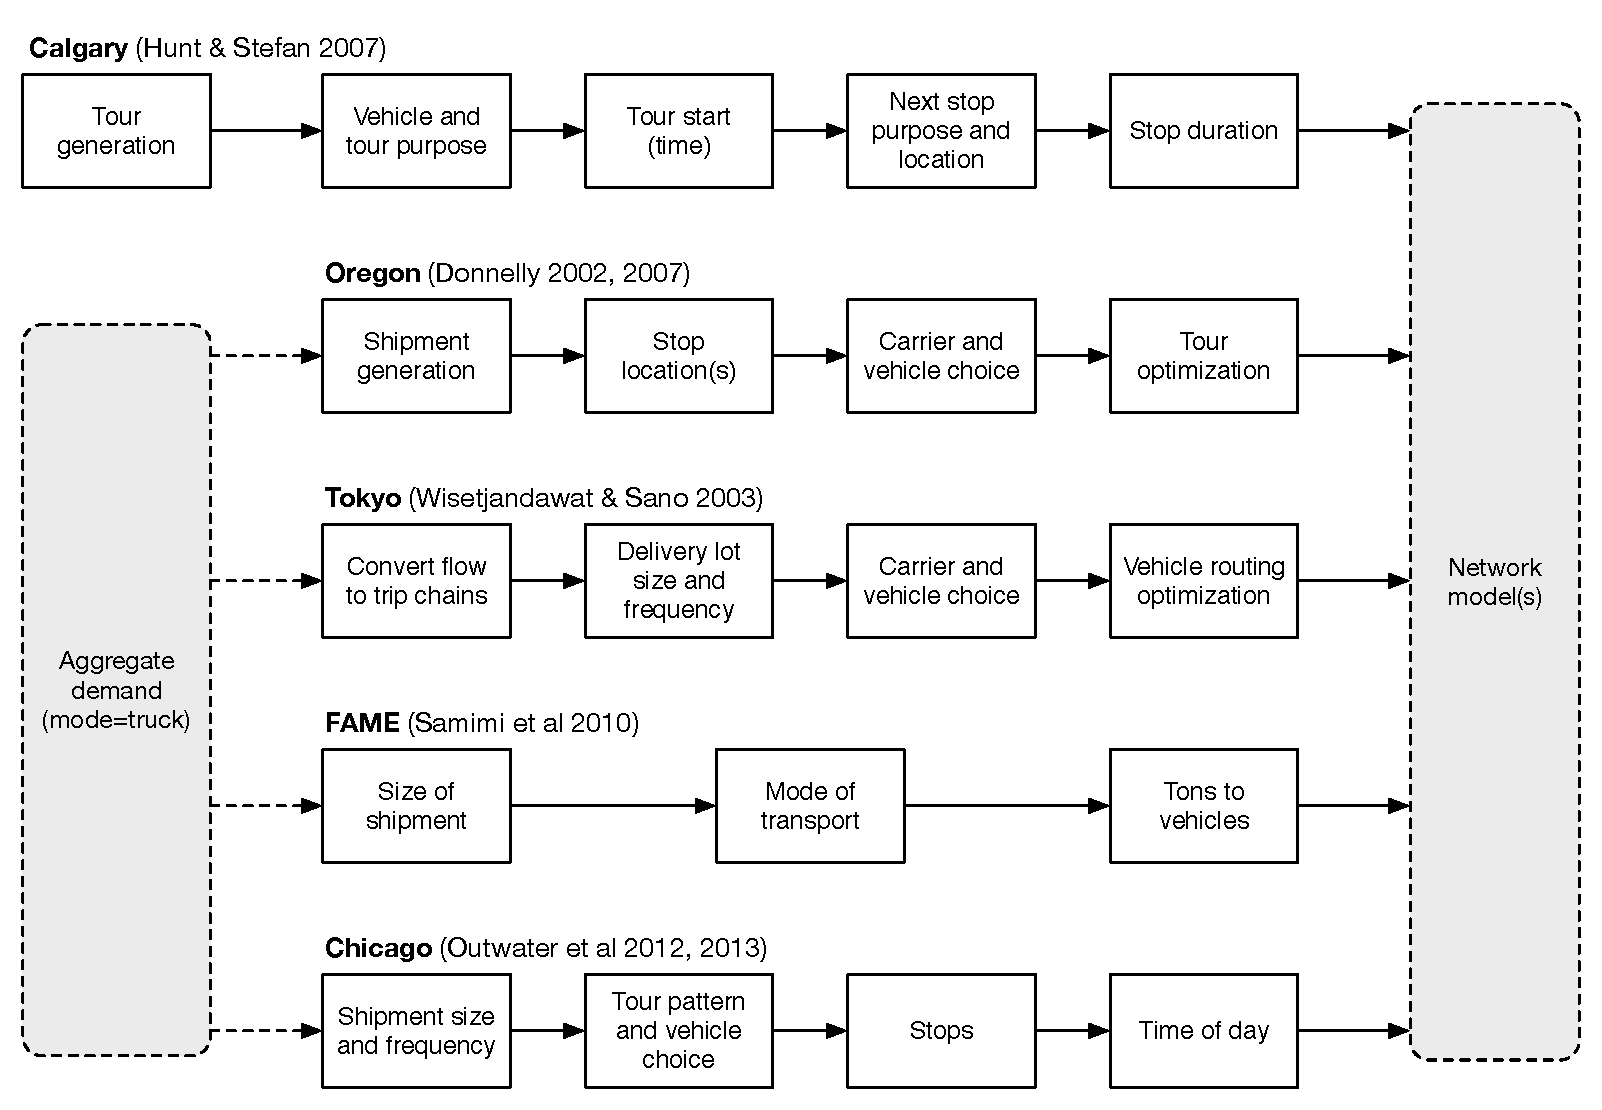
\includegraphics[width=6.5in]{figures/truck-tour-models}
\caption{Summary of known operational truck tour models}
\label{fig:ct-truck-tour-models}
\end{figure}

The convergence of approaches used to simulate truck tours lends validity to the emphasis in the initial design of the CT module, as well as the methodology used to construct them. The operational models profiled in Figure \ref{fig:ct-truck-tour-models} all map commodity flows to discrete shipments that are routed on trucks of different types, an approached followed in the CT module. The CT implementation still relies upon a combination of synthetic and asserted data, for establishment and truck operator surveys have yet to be conducted in Oregon. However, the resulting models can be calibrated to replicate observed counts patterns across the state.

It might be argued that truck tour patterns are more important in urban modeling, whereas the emphasis should be on intercity flows in the statewide model. Such flows are predominately freight movements made using tractor-trailer combinations. It is argued that the distinction between local and long-distance trips is arbitrary, and probably less distinctive than for person travel. This is especially true in the Willamette Valley, which likely represents a single market for many firms, rather than collection of smaller but distinct urban markets. 

\subsection{Large variances inherent in firm and freight behaviors}\label{sec:ct-large-variances}

The scope of the CT module is as ambitious as the PT module. While fewer in number than persons or households, firms differ by their industrial classification, size (in employees, as well as floorspace consumption), location, ownership, position(s) within supply chains, and market areas. There are tremendous variations in activities and levels of freight generation even by otherwise similar firms within the same industry. The use of private versus for-hire carriers results in significant differences in travel behavior, as well as helping to define the firm's market area and share. An analysis of the relationship between tonnage and value from Commodity Flow Survey (CFS) microdata reveals very large coefficients of variation, as does similar analyses of mean trip length. Even the total tonnage of commodities shipped regressed against employment by county or FAF region reveals variances much larger than mean values. These variances are much larger than comparable measures obtained from person travel surveys. 

Such findings influenced the design of the CT module. Closed-form deterministic models, long used in person travel forecasting models, are better suited for modeling behaviors with strong central tendencies. Simulation modeling, on the other hand, has been more widely used for modeling populations with large variances, which are better represented by non-uniform probability distributions. The ability to explicitly represent the non-linear and multimodal distributions found in the data prompted the decision to use a microsimulation approach for the CT module. It is also easier to handle different levels of spatial and temporal resolution within such a framework. Some of the distributions of key data do not follow ideal forms, making sampling from them more straightforward and easy to adjust during calibration than complex behavioral models.

The large variances in the data, coupled with the smaller volume of commercial travel relative to person flows within SWIM2, must also temper our expectations with respect to model accuracy. In corridors with high freight volumes we will obtain the benefit of measures of central tendency, even when the mean and median values are not close together. Smaller flows, whether on links or between zone pairs, are likely to be more divergent from a mean value, or single truck counts, than we would expect for auto flows or all types of traffic combined. There are no widely accepted accuracy targets for freight models. However, the addition of constants or arbitrary adjustment factors in order to create the illusion of closer fit to observed counts is highly discouraged. It provides false confidence in the model results, and masks patterns that the analyst should consider when interpreting the results. The results of the CT validation can therefore be compared to comparable models elsewhere, but should not be measured against how well the person travel model performs by comparison.

\subsection{Freight Analysis Framework (FAF) integration}\label{sec:faf-integration}

The original CT module used data from aggregated summaries of the 1997 and 2003 Commodity Flow Surveys to estimate commodity flows by mode of transport between Oregon and other states. This enabled the SWIM2 model to be placed within a national context with respect to commodity and freight flows, without the need for maintaining a national freight model. The need for such a placeholder was dramatically reduced, and eventually eliminated, as the Freight Analysis Framework (FAF)\footnote{\url{http://ops.fhwa.dot.gov/FREIGHT/freight_analysis/faf/index.htm}} evolved as capable of fulfilling that role. The current version of CT relies heavily upon the FAF to depict long-distance freight flows.

The FAF was originally developed by FHWA as a tool for federal policy analyses. The first version was created in 1997-99 using existing ``off the shelf'' data from both the public and private sectors. Included in the latter were economic forecasts for each state, as well as some third-party products such as the Reebie Transearch data. It represented a proof of concept for a national freight model, as well as providing immediate estimates that could be used by the USDOT to assess proposed corridors of national significance. The FAF hqs evolved considerably since then, with major versions coinciding with the release of each new CFS in 2003, 2007, 2012, and 2017. The latest release, Version 5.4.1 at the time of this writing, represents two decades of continual development and improvement in data quality and analytical methods. 

The current FAF provides a far more holistic picture of freight flows than the CFS alone. Data from several sources are used to develop the database:
\begin{itemize}
\item Commodity Flow Survey (both publicly available and microdata),
\item Vehicle Inventory and Use Survey (VIUS; discontinued after 2002 survey),
\item Carload Waybill Sample data collected by the Surface Transportation Board (both spatially aggregated public use and detailed data available only to government agencies),
\item Domestic and international Waterborne Commerce data collected by the U.S. Army Corps of Engineers,
\item Air freight movement data compiled by the Bureau of Transportation Statistics, and
\item Foreign trade statistics compiled by the U.S. Department of Commerce.
\end{itemize}

Most users of the FAF find it superior to using the CFS alone. The improved transparency, greater level of detail, availability of forecasts, and online documentation are significant benefits associated with the FAF. The data are still too spatially coarse to be used in statewide modeling, much less at the urban scale. It is widely acknowledged that the FAF under-estimates trips within urban areas, which is not surprising given that it is constructed from national data sources.

The FAF is not so much an analytical framework --- a phrase that suggests underlying models --- as it is a commodity flow database. There are no user-accessible analytical methods or products embedded within the FAF. No mode choice model is included, nor are any other policy-sensitive models. As a consequence, existing patterns and trends are extrapolated into the future. This can hardly be construed in a negative light, considering that existing choices and preferences remain also invariant in most person travel demand forecasts. Moreover, the amount of progress made over the past several versions of the FAF is remarkable nonetheless. Perhaps most importantly, the FAF can be used with statewide or national freight models in a far easier manner than the CFS alone.

Unlike the CFS upon which it is built, recent versions of the FAF provide a comprehensive database of freight flows rather than limited static tabulations. Two principal databases are produced:
\begin{itemize}
\item Origin-destination flows of annual freight by commodity and mode of transport, measured in tons, value, and ton-miles. These are provided at the county level or international gateway for users within the USDOT, and at the CFS region or international gateway level for all other users.
\item Estimates of flows on major routes and segments of highways, by mode of transportation. A range of tonnage is provided at the route level, while truckload equivalents and tons of truck-carried freight are available for segments. Additional attributes are available to USDOT users, such as the commodity and origin-destination data.
\end{itemize}

\noindent These data are available for the base year (2017 for Version 5) and for forecasts in five-year intervals from 2020 through 2050. The economic forecasts used to create the 2020--2050 forecast series are not disclosed, nor are tools provided to modify their imbedded assumptions. Thus, one cannot test the effect of different economic futures using the FAF. That said, each version of the FAF has included low, mid-range, and high growth economic forecasts that incorporate the best available information at the time. Version 5 represents a significant improvement in this regard, for it incorporates data to more accurately portray the effects of recent economic conditions on freight flows.

One lingering limitation of the FAF is its coarse level of spatial resolution. For internal use within the USDOT the data are available at the county level. The data are substantially more aggregated when released to all other users, at the FAF region level. While the data are still more aggregate in nature than many state and local planners need, it represents a significant improvement over the CFS. Different teams have developed approaches to disaggregate flows between FAF regions to flows between counties or even flows between urban model zones. Most approaches use one or both of two methods:
\begin{itemize}
\item \textit{Multiple regression:} Commodity-specific flows into and out of a FAF region are used as the dependent variable and employment by type are used as the independent variable. Linear multiple regressions are used to estimate parameters that help explain which employment types generate and attract flows of a given commodity. These parameters are used to disaggregate to smaller zones within a FAF region. 
\item \textit{Input-output coefficients:} Such coefficients describe which commodities are consumed and produced by a given industry. Multiplying employment by type with the corresponding IO coefficients generates a weight for each zone within a FAF region to allocate from the latter to the former.
\end{itemize}

\noindent Both methodologies have been applied widely and appear to generate comparable results, at least at the level of daily network assignments. The former approach has the limitation that parameters are estimated based on large FAF regions with a fairly homogeneous industry mix across the country. The latter approach relies on input-output coefficients that commonly are estimated as dollar flows, while freight flows usually are processed as weight-based flows. Because Oregon-specific IO coefficients are available from the AA module this approach is used in the CT module.

\section{Quantity definitions and model building blocks}

The CT model is largely compatible with the other SWIM2 modules with respect to basic definitions and concepts, with a few notable exceptions.

\subsection{Local versus long-distance travel}

An artificial distinction is often made between local versus long-distance truck trips, largely because the CFS and FAF only include the latter. The definition has changed over the past 30--40 years, but the distance cutoff for inclusion in the CFS currently is 50 miles. This distinction was used in previous versions of CT, but relaxed in the current one. Survey data from other places were used to portray the trip distance frequency distribution for local trucks, whose trips often extend to 100 miles without leaving the local area. We do not assume that such trucks are adequately represented in the FAF data, although some unquestionably are. Our empirical testing suggests that estimates from both sources can be used to portray travel within the distance ranges they overlap without distracting from model performance. Moreover, many of the local truck trips do not involve freight movements, so would not be double-counted in any case.

\subsection{Geographic coverages}\label{sec:ct-geographic-coverages}

The world outside of Oregon is represented by FAF regions, which are aggregations of counties within the USA and countries or world regions outside of it. Three of the 132 domestic FAF regions are contained within the SWIM2 halo:
\begin{itemize}
    \item FAF region 411 includes the Oregon counties within the Portland Metropolitan Statistical Area (MSA)
    \item FAF region 419 includes the remaining counties within Oregon
    \item FAF region 532 includes the Washington counties within the Portland MSA
\end{itemize}

Some FAF regions correspond to MSA boundaries\footnote{MSAs covering multiple states are coded as separate regions in each state. For example, the Chicago region is represented by FAF regions in Illinois and Indiana.}, with areas outside of them classified as ``remainder of state.'' There are also eight world regions outside the USA, which describe the distal end of imports and exports.\footnote{This information is used to portray the foreign origins and destinations for traffic through the Port of Portland, but are otherwise not used in the SWIM2 system.} Canada is unfortunately represented by a single FAF region, although the domestic FAF region it crosses the border is coded in the data. Thus, neither the data nor the CT model can distinguish between flows between Oregon and British Columbia (BC) versus flows to other provinces that merely cross the border there.

The CT module operates at the alpha zone level within Oregon.\footnote{Counties can optionally be used to constrain the allocation of flows to alpha zones. This functionality might be useful in model calibration, or if the analyst wished to force assumed economic and commodity flow growth into certain areas of the state.} Because only Oregon and the halo are represented in the SWIM2 network the Interstate flows generated by CT are routed through the external zones shown in Figure \ref{fig:swim2-external-zones}. A program was written that extracts the minimum time path from the centroids of FAF regions\footnote{We defined the centroids as the center of the MSA for FAF regions defined as such, and intersection of Interstate highways for regions encompassing the remainder of the state.} from the Google Maps API, and associates the path with the corresponding external gateway in Figure \ref{fig:swim2-external-zones}. The definitions of the external zones and the 2020 truck counts associated with them are summarized in Table \ref{tab:swim2-external-zones}.

\begin{figure}[!t]
\centering
\fbox{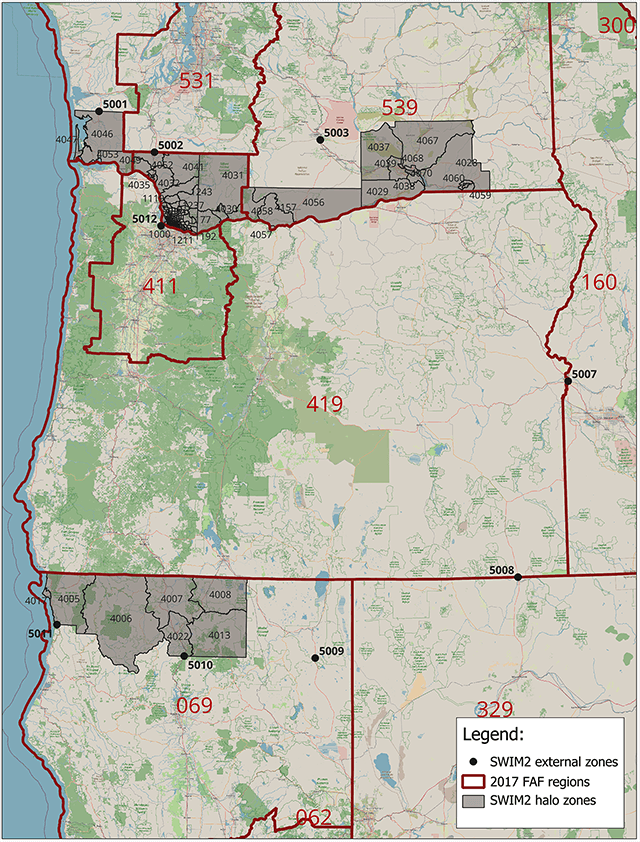
\includegraphics[width=5.5in]{figures/new-external-zones.png}}
\caption{SWIM 2.6 external zones}
\label{fig:swim2-external-zones}
\end{figure}

\begin{table}
\centering
\caption{SWIM2 2.6 external zone definitions}
\label{tab:swim2-external-zones}
\begin{threeparttable}
\begin{tabular}{cllr}
\hline
Zone\tnote{a} & Location & Route & 2020 AADTT\tnote{b} \\
\hline
5001 & Border of Pacific and Gray's Harbor Counties, WA & US-101 & 311 \\
\gray 5002 & Border of Cowlitz and Lewis Counties, WA & I-5 & 6,265 \\
5003 & Union Gap, WA & I-82 and US-97 & 2,700 \\
\gray 5004 & Franklin County WA-Oregon border & US-385 & 1,194 \\
5007 & Oregon-Idaho state line & I-84 & 2,258 \\
\gray 5008 & Oregon-Nevada state line & US-95 & 264 \\
5009 & Border of Modoc and Lassen Counties, CA & US-395 and OR-39 & 130 \\
\gray 5010 & Border of Siskiyou and Shasta Counties, CA & I-5 & 3,465 \\
5011 & Border of Del Norte and Humboldt Counties, CA & US-101 & NA\tnote{c} \\
\gray 5012 & Port of Portland marine port & N. Marine Drive & NA \\
\hline
\end{tabular}
\begin{tablenotes}
\footnotesize
\item[a] Gaps in numbering reflect external zones deprecated in SWIM 2.6 update
\item[b] Average annual daily truck traffic (AADTT) flows are directional (i.e., the flows shown occur in each direction)
\item[c] The truck flows across this external zone are so small that it is not included in the CT analyses
\end{tablenotes}
\end{threeparttable}
\end{table}

The Port of Portland's marine port is defined as external zone 5012. The remaining air and marine ports are defined by the alpha zone encompassing them. It was assumed that all air cargo from or to Oregon were routed through the Portland International Airport. Marine traffic moving through the Portland MSA was assumed to move through the Port of Portland, while similar traffic elsewhere in Oregon was assumed to move through the Port of Coos Bay.\footnote{The Port of Astoria primarily serves passenger flows. Their cargo volume is very small, enabling us to ignore it. However, the analyst should revisit this assumption if major cargo handling through the Port of Astoria is tested in future scenarios.} 

Rail origins and destinations within Oregon are coded to FAF regions. Confidential data from the Surface Transportation Board's Carload Waybill Sample (CWS) were used to identify the specific Standard Place Location Codes (SPLCs) associated with such flows. Most SPLCs were coded to county level, but easily precisely located by searching for rail yards using satellite imagery. It was found that seven rail facilities account for 90 percent of the rail traffic beginning or terminating in Oregon. These data were used to develop rail accessibility measures that enabled us to code the origin or destination FAF region within Oregon to specific alpha zones.

\subsection{Commodity and vehicle definitions}\label{sec:ct-commodity-truck-def}

Commodities are coded using the two-digit Standard Classification of Transportable Goods (SCTG) codes, which are also used in the AA module. These codes are shown in Table \ref{tab:sctg-codes}. The data included in the FAF is also coded to SCTG, as are CFS data from 2002 onward. The CWS commodities are coded to seven-digit Standard Transportation Commodity Codes (STCC)\footnote{\url{https://www.railinc.com/rportal/standard-transportation-commodity-code}}, and converted to two-digit SCTG codes using a previously developed concordance.

\begin{table} 
\centering
\caption{Standard Classification of Transportable Goods (SCTG) codes}
\label{tab:sctg-codes}
\begin{tabular}{clcl}
\hline
Group & Description & Code & Description \\
\hline
A & Agricultural & 01 & Live animals and fish \\
& products and & 02 & Cereal grains (includes seed) \\
& fish & 03 & Agricultural products, not elsewhere classified \\
& & 04 & Animal feed, eggs, honey, and other products of animal origin \\
& & 05 & Meat, poultry, fish, seafood, and their preparations \\
\gray B & Grains, alcohol, & 06 & Milled grain products and preparations, and bakery products \\
\gray & and tobacco & 07 & Other prepared foodstuffs, fats and oils \\
\gray & products & 08 & Alcoholic beverages and denatured alcohol \\
\gray & & 09 & Tobacco products \\
C & Stones, & 10 & Monumental or building stone \\
& non-metallic & 11 & Natural sands \\
& minerals, and & 12 & Gravel and crushed stone (excludes dolomite and slate) \\
& metallic ores & 13 & Other non-metallic minerals not elsewhere classified \\
& & 14 & Metallic ores and concentrates \\
\gray D & Coal and & 15 & Coal \\
\gray & petroleum & 16 & Crude petroleum \\
\gray & products & 17 & Gasoline, fuels, and ethanol \\
\gray & & 18 & Fuel oils (includes diesel, Bunker C, and biodiesel) \\
\gray & & 19 & Other coal and petroleum products, not elsewhere classified \\
E & Basic chemicals,& 20 & Basic chemicals \\
& chemical and & 21 & Pharmaceutical products \\
& pharmaceutical & 22 & Fertilizers \\
& products & 23 & Other chemical products and preparations \\
& & 24 & Plastics and rubber \\
\gray F & Logs, wood & 25 & Logs and other wood in the rough \\
\gray & products, and & 26 & Wood products \\
\gray & textiles and & 27 & Pulp, newsprint, paper, and paperboard \\
\gray & leather & 28 & Paper or paperboard articles \\
\gray & & 29 & Printed products \\
\gray & & 30 & Textiles, leather, and articles of textiles or leather \\
G & Base metal and & 31 & Non-metallic mineral products \\
& machinery & 32 & Base metal in primary or semi-finished forms and finished basic shapes \\
& & 33 & Articles of base metal \\
& & 34 & Machinery \\
\gray H & Electronics, & 35 & Electronics, electrical equipment and components, and office equipment \\
\gray & motorized vehicles, & 36 & Motorized and other vehicles (includes parts) \\
\gray & and precision & 37 & Transportation equipment, not elsewhere classified \\
\gray & instruments & 38 & Precision instruments and apparatus \\
I & Furniture, mixed & 39 & Furniture, mattresses, lighting, and illuminated signs \\
& freight, and & 40 & Miscellaneous manufactured products \\
& miscellaneous & 41 & Waste and scrap (excludes of agriculture or food) \\
& products & 43 & Mixed freight \\
\hline
\end{tabular}
\end{table}


The FAF truck flows are grouped into five truck types, as shown in Table \ref{tab:faf-truck-configuration} \citep{battelle11}. These are collapsed to single and multi-unit trucks (SUT and MUT, respectively) for traffic assignment. It is readily acknowledged that there is considerable ambiguity in the definition of trucks, for many commercial vehicles are passenger vans and pickup trucks, which are not included in the categories described above. They cannot be separated from identical privately owned vehicles in count data. Moreover, such privately owned vehicles are sometimes also used for commercial purposes, further blurring the distinction between them. The FAF definitions were used to ensure compatibility with that data source, whereas other data sources used to develop CT only differentiated between SUT and MUT (and sometimes light goods vehicles [LGVs] to represent vans and pickup trucks).

\begin{table}
\centering
\caption{FAF truck configurations}\label{tab:faf-truck-configuration}
\begin{tabular}{cl}
\hline
Category & Description \\
\hline
SU & Single-units trucks \\
\gray TT & Single-unit truck plus trailer combinations \\
CS & Tractor plus semi-trailer combinations \\
\gray DBL & Tractor plus double trailer combinations \\
TPT & Tractor plus triple trailer combinations \\
\hline
\multicolumn{2}{l}{\footnotesize Source: \cite{battelle11}}
\end{tabular}
\end{table}

During local truck generation (\S\ref{sec:ct-tour-generation}) trucks are further classified as being privately owned or for-hire, for their tour characteristics and assumptions about ability to pick up backhauls are quite different in most cases. This distinction is referred to as \textit{carrier type} in the CT model. The final list of discrete truck trips includes this and other facets of information, but they are not retained in the user classes used in traffic assignment.

\subsection{Zonal activity estimates}

Zonal estimates of employment by industry sector have traditional been used as surrogates for firms to define the points of production, exchange, and consumption within urban and statewide freight models. A firm synthesis, comparable to the synthetic population generator (SPG) module described in Chapter 4 in the \textit{SWIM2.5 Model Delivery Report}, was considered for this version of the CT module. It was felt that would improve the representation of business-to-business (B2B) transactions, and enable the inclusion of other firm attributes in the CT models. Several methodologies exist for creating such synthetic firms, ranging from older but likely still viable approaches proposed by \cite{chiang76} to more elegant firmographic models \citep{moeckel06, pagliara13}. The barriers to building such a model for the base year are probably minor, but questions remain about whether such approaches convey significant benefits and appropriate ways generate such estimates in the future. It was decided to retain full consistency with AA in this regard, by using its employment estimates at the alpha zone level, by the sectors defined in Table 2.3 (page 13) in the \textit{SWIM2.5 Model Delivery Report}.

Many service stops are made at households, as well as a growing number of freight deliveries. The total number of households per alpha zone are summarized from the synthetic population for the simulated year. It is supposed that younger professionals are more likely to use electronic commerce than older individuals, and that higher-income households consume more than lower-income households of the same size. However, no hard disk exists on which to base such conclusions. Thus, total households per zone are used at the present time in the model, although it will be simple to stratify them by income or other measures in the future.

\section{Component models}

The CT module simulates the demand for local and long-distance travel made in commercial vehicles within the SWIM2 modeled area. It consists of several submodels, as shown in Figure \ref{fig:ct-high-level}. The CT modules requires data from the current simulation from the AA module as well as several runtime properties and model parameters. It produces tour and trip lists for discrete commercial vehicles that can be aggregated into multiclass trip matrices by period of the day for network assignment. In between are submodels that simulate local and long-distance truck trips, shown on the top and bottom rows, respectively, of Figure \ref{fig:ct-high-level}. Each of these submodels are described in the sections that follow.

\begin{figure}
\centering
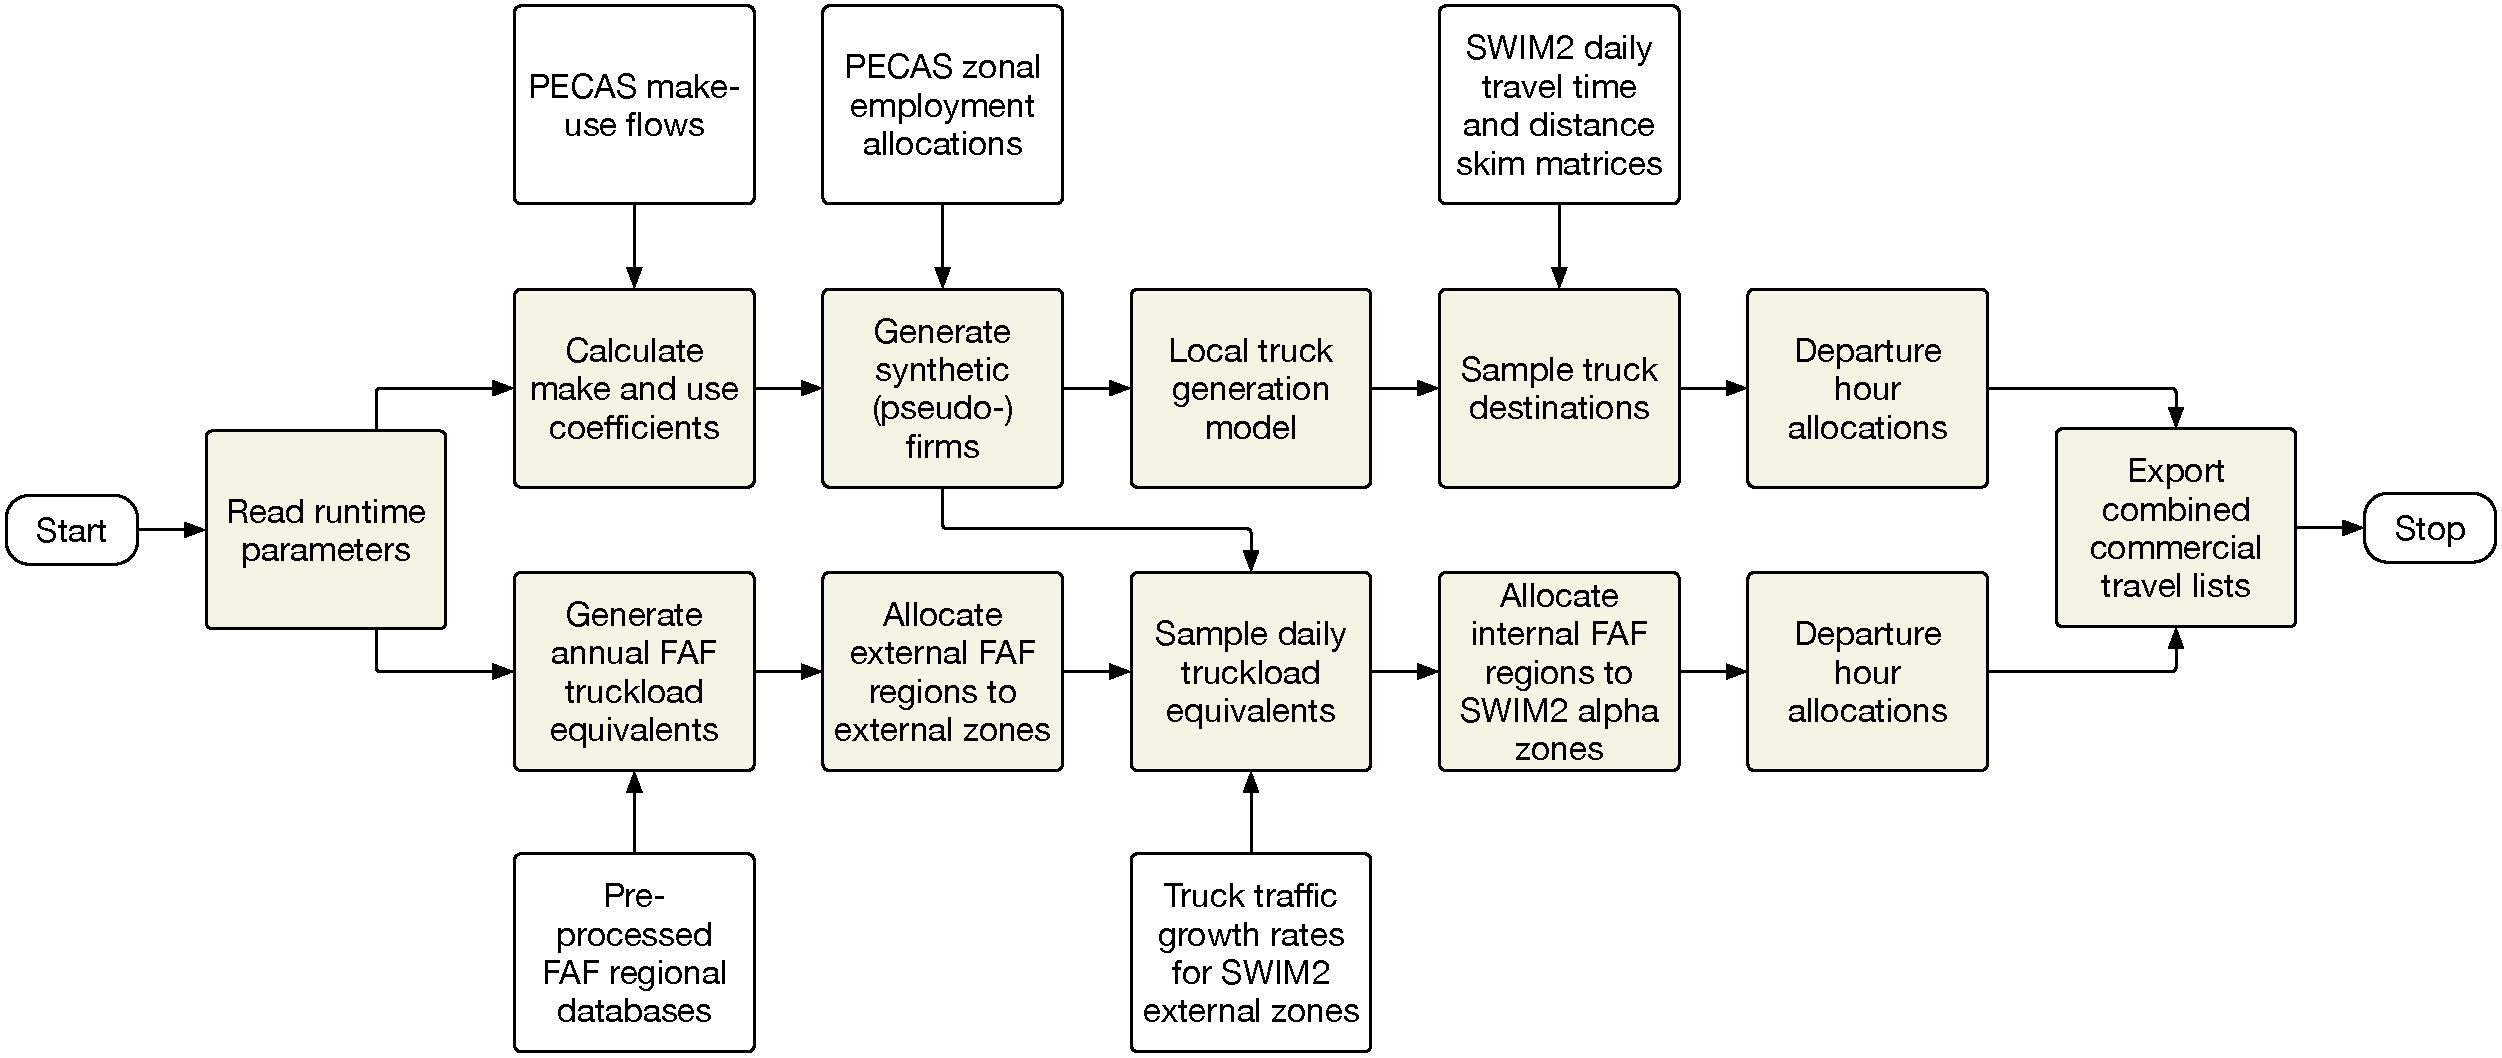
\includegraphics[width=6.25in, trim=0mm 10mm 0mm 0mm]{figures/ct-high-level}
\caption{High-level schematic of the CT module components and interoperability}
\label{fig:ct-high-level}
\end{figure}

Three approaches to generating commercial vehicles were tested during the development of the CT module:
\begin{itemize}
    \item Directly assigning truckload equivalents of the AA production-consumption flows (original CT design)
    \item An aggregate trip-based truck model
    \item A multi-agent revised tour-based truck model
\end{itemize}

\noindent The direct assignment option was abandoned after several different attempts, as discussed in \S\ref{sec:ct-swim-integration}. The trip and tour-based approaches for local travel were coupled with allocation of the FAF flows to represent long-distance freight movements within and through Oregon. The trip and tour-based truck models were extensively tested and found to produce comparable results. The total number of trips generated in the former were used to constrain the number of tours generated in the latter, providing a better fit to observed data. The truck tour model was selected for adoption due to it more flexible design and ability to support a wider range of analytics.

The sections that follow describe each of the component models shown in Figure \ref{fig:ct-high-level}. The modeling of long distance flows using the FAF are described in the next three sections, followed by a discussion of the local travel models. 

\subsection{Long-distance truck modeling}\label{sec:long-distance-models}

The process for coverting the annual FAF flows into daily truckload equivalents is shown in the top row of Figure \ref{fig:ct-high-level}. The primary input to the process is the FAF regional database of commodity flows. This file is available for download on the FAF web page.\footnote{\url{https://ops.fhwa.dot.gov/freight/freight_analysis/faf/}} A preprocessor written in RMarkdown\footnote{\url{https://rmarkdown.rstudio.com}} is included in the \verb|data-raw| folder of the \verb|tlumip/swimctr| code repository\footnote{\url{https://github.com/tlumip/swimctr}} that converts the database distributed by FHWA into the format used by the CT module. The preprocessor extracts flows that have one or more trip ends within Oregon or passes through the state. Travel times outside of the SWIM2 halo are added, and some categorical variables are mapped from integer levels to alphameric strings. This preprocessing needs to be completed only once when each new FAF version is released. The reformatted database is also stored in the \verb|data-raw| folder of the \verb|tlumip/swimctr| repository.\footnote{Note that the FAF version currently used by the CT module may be one or more minor versions away from the most current version on the FHWA website. The user can decide which version to retain in the code repository. Best practices dictates updating minor versions when released. Major versions (e.g., Version 5 to 6) should be carefully checked and tested before inclusion in the CT module.}

The translation of the preprocessed FAF data into daily truck flows is accomplished in several steps:
\begin{enumerate}
    \item The commodity flows in the preprocessed FAF database, measured in annual dollars and tons, are converted into annual truckload equivalents for the current simulation year. Commodity flows from the closest year in the FAF data to the SWIM2 simulation year are extracted in this step. The process used for this transformation is described in the next section. The FAF only includes a single truck class, requiring the additional step of selecting one of the five truck types shown in Table \ref{tab:faf-truck-configuration}. The truck type allocation factors, binned by trip length\footnote{The truck allocation factors are applied based on the total length of the trip (i.e., distance between FAF region centroids) coded in the FAF data, not just the distance traveled within the SWIM2 halo.}, are shown in Figure \ref{fig:truck-allocation-factors}.

\begin{figure}
\centering
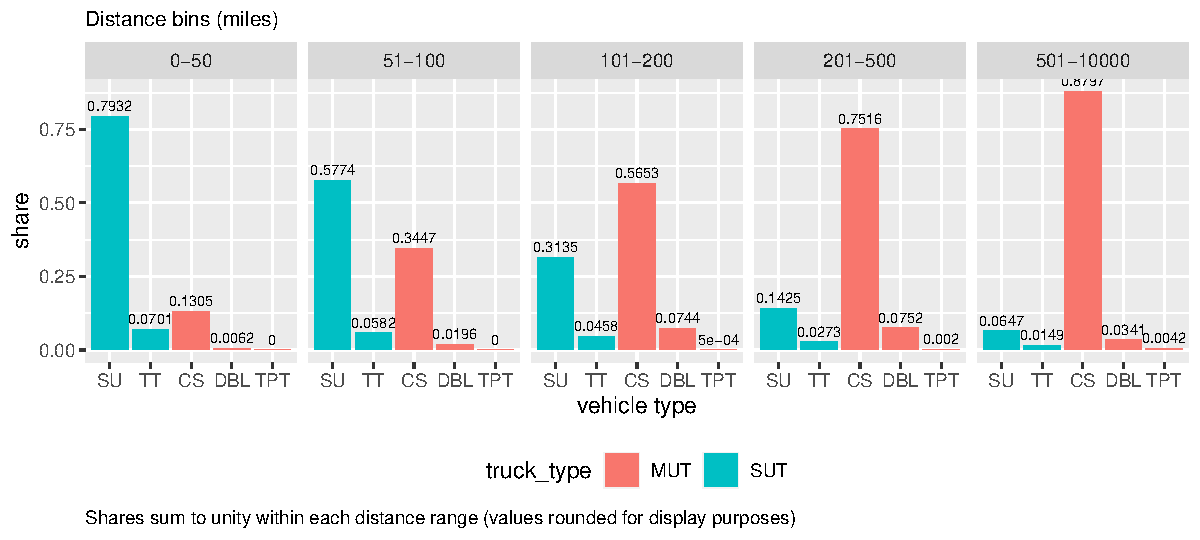
\includegraphics[width=6.6in]{figures/graph-truck-allocation-factors.pdf}
\caption{FAF truck allocation factors}
\label{fig:truck-allocation-factors}
\end{figure}

    \item Trip ends in FAF regions outside of the SWIM2 halo are allocated to SWIM2 external zones using shortest travel time paths on the National Highway Planning Network (NHPN).\footnote{\url{https://data-usdot.opendata.arcgis.com/datasets/usdot::national-highway-planning-network/}} The accuracy of these travel times were compared to comparable values generated between the same trip ends in Google Maps. Because more than one path between FAF regions was possible up to three plausible routes were defined. The share of trips $S$ allocated to each route $r$ was based upon an inverse travel time function of travel time $t$:
    \begin{equation}
    S_r = 1 / {t^3}
    \end{equation}
    An example of the calculation of route probabilities between Bozeman and Portland is shown in Table \ref{tab:route-alloc-example}. A route is sampled with the normalized weight $N_r$ for each truckload equivalent simulated in the previous step, replacing the external FAF region with the SWIM2 external region the sampled path passes through. Longer routes have a lower probability, but not zero, chance of being selected. When applied to annual truckload equivalents a large number of trucks are allocated to each plausible route.
    \item Daily truck trips are sampled from the annual truck trips by trip direction. The FAF flow directions are coded with respect to the SWIM2 modeled area (SMA):
    \begin{enumerate}
        \item[a.] Internal trips have both origin and destination within the SMA
        \item[b.] Inbound trips have only the destination within the SMA
        \item[c.] Outbound trips have only the origin within the SMA
        \item[d.] Through trips have neither origin nor destination within the SMA
    \end{enumerate}
    The inbound, outbound, and through trips are sampled such that their sum equals the observed or asserted average annual daily truck traffic (AADTT) volumes at each SWIM2 external zone. The observed values are year 2020 counts from automated traffic recorders near the Oregon border for SWIM2 external zones on the border and from counts culled from traffic count databases in adjacent states. These are summarized in Table \ref{tab:swim2-external-zones}. A single value of $1 \div 260 = 3.85e-03$ was derived to scale the daily internal trips. Note that there are $52 \times 5 = 260$ workdays in a year. This target, arrived at through iterative comparison with observed counts, appears quite intuitive.\footnote{It is acknowledged that long-distance trucks operate every day of the year, including holidays. However, shorter distance trucks -- internal FAF trips -- likely serve local markets that probably do most of their distribution and deliveries during the work week.}
    \item The internal trip ends---those to and from the three FAF regions within the SMA (\S\ref{sec:ct-geographic-coverages})---are next allocated to alpha zones within each of the three regions. Because discrete trucks are being simulated a sampling approach to destination choice is preferred to an aggregate gravity model approach. The zonal employment $E$ by sector $s$ and make-use coefficients from the AA module run in the simulation year are used to generate a \textit{production attractiveness score} $P$ for each zone $z$ within each internal FAF region $r$. For origins the make coefficients $M$, which are the proportions consumed from each sector $s$ required to produce one unit of output\footnote{The resulting make and use coefficients sum to unity, obviating the need for normalizing them prior to sampling.}, are used to scale the employment estimates:
    \begin{equation}
    P_{irs} = E_{irs} \times M_s, \; i \in r, r \in (411, 419, 532)
    \end{equation}
    The internal trip end $z$ is sampled with replacement using the weighted scores $P_{irs}$ for each trip record. This replaces the internal FAF region origin coded on the trip record. Similarly, for destinations coded in internal FAF regions a \textit{consumption attractiveness score} $C$ is constructed using the AA use coefficients $U_s$, which define the production inputs reqiured to produce a single unit of output:
    \begin{equation}
    C_{irs} = E_{irs} \times U_s, \; i \in r, r \in (411, 419, 532)
    \end{equation}
    At the end of this process all of the FAF records are coded to SWIM2 alpha zone origins and destinations.
    \item Departure times are appended to each trip in the final step of processing the FAF data. Many trips from outside the SMA begin before the simulation clock starts, especially for travel from distant states. Their initial departure time is unknown. However, they effectively enter the simulation at the SWIM2 external zones, and only their movements within the SMA are represented. Thus, assigning departure times based on observed peaking characteristics within Oregon. The observed temporal distributions are shown in Figure \ref{fig:ct-trip-departure-times}. These distributions, indexed by truck type, are sampled to assign a departure hour, with the minute within each hour randomly sampled. This approach is adequate, given that the trips will be aggregated into assignment periods of several hours each.\footnote{}
\end{enumerate} 

\begin{table}
\centering
\caption{Example FAF route allocation between Bozeman and Portland}
\label{tab:route-alloc-example}
\begin{tabular}{lrrr}
\hline
Route & Travel time (hr) & $S_r$ & $N_r$ \\
\hline
Via I-90 & 11.0 & 7.513e-4 & 0.4581 \\
\gray Via I-90 and US-12 & 12.75 & 4.825e-4 & 0.2941 \\
Via I-84 & 13.5 & 4.064e-4 & 0.2478 \\
\hline
Sum & & 1.640e-3 & 1.0000 \\
\hline
\end{tabular}
\end{table}

The process translates the aggregate flow matrices to discrete daily trucks, which are allocated to SWIM2 alpha zones for the trip ends within Oregon. The distal trip ends are coded to the external zones at the edge of the halo (Figure \ref{fig:swim2-external-zones}).

\subsection{Creation of FAF truckload equivalents}

The FAF commodity flow data are reported in annual tonnage and value flows rather than discrete trips. No information is provided about the number of trucks used to deliver the shipments reported in the FAF. A process developed by Oak Ridge National Laboratory (ORNL) was developed during FAF Version 3 to map tonnages reported in the FAF to truckload equivalents. The three-step process first divided the tonnage by vehicle type and then by trailer type. The last step in the ORNL process generated empty truck flows, which are not accounted for in the FAF. The ORNL process applied to Oregon resulted in a large percentage of trucks exceeding the 80,000 pound gross vehicle weight\footnote{The GVW includes the weight of the empty vehicle, fuel, passengers, and cargo.} (GVW) allowed within Oregon. It was also at odds with limited weight data collected early in the TLUMIP work that revealed a uniform distribution of truck weights rather than the majority greater than 75,000 pounds, with many implausible GVW estimates.

The 2002 VIUS microdata was evaluated as an alternative method for translating tonnage to truckload equivalents. The weights were reported in only three very broad intervals and relied upon respondents estimates rather than measurements. These were deemed unsuitable for the purpose at hand. 

The 2012 Canadian CFS, which included detailed intercept surveys of intercity trucks, proved a much more robust source. The respondents reported not only commodities carried but the previous and next stops in addition to both truck and cargo origin and destination. Moreover, the survey captured both loaded and empty trucks passing 212 highway and arterial survey locations in the Canadian province of Ontario. In contrast to U.S. data sources, the intercepted trucks were weighted using portable weigh-in-motion equipment in most instances. 

It was straightforward to build histograms of payload weight from the Canadian data, shown in Figure \ref{fig:cvs-weight-distributions}. There were an insufficient number of observations for triple-trailer trucks (TPT), so the double-trailer truck distribution was duplicated for them. Given the very small incidence of TPT trucks (see Figure \ref{fig:truck-allocation-factors}) it is unlikely to skew the truckload equivalencies.

\begin{figure}[!tb]
\centering
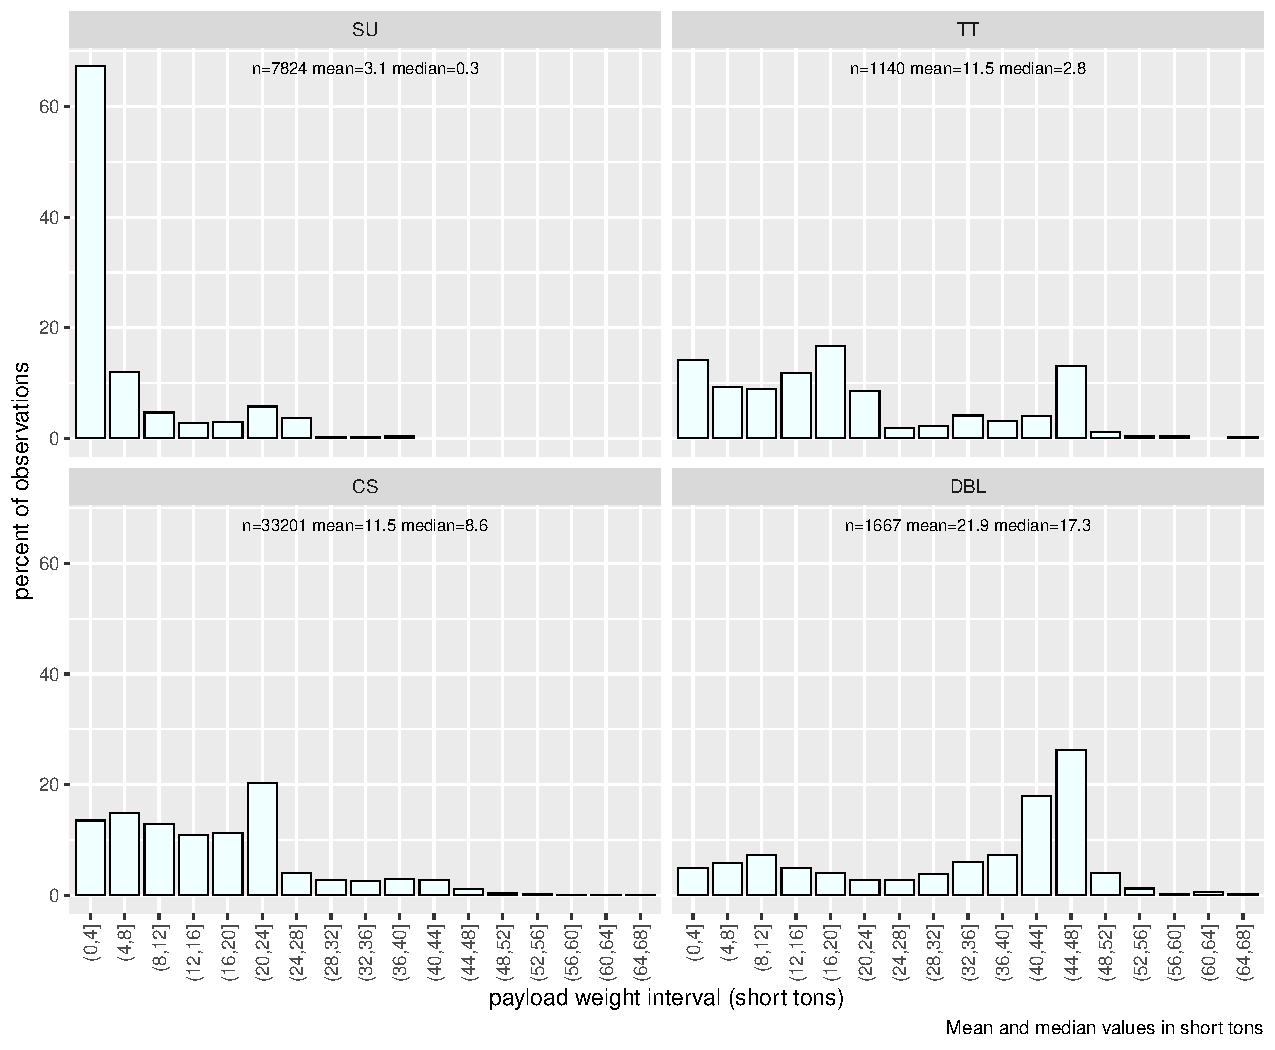
\includegraphics[width=6in]{figures/graph-cvs-payload-distributions.pdf}
\caption{2012 Canadian CFS payload weight distributions by truck type}
\label{fig:cvs-weight-distributions}
\end{figure}

Annual truckload equivalents are created by sampling the number of trucks required to carry the annual tonnage reported on each FAF record for the simulation year. The truck types are sampled first for each simulated truck so that the appropriate weight ranges for each truck are sampled. The sampling continues for each FAF commodity flow record until enough trucks have been generated to move the reported annual tons. About 17.8 million annual trucks flowing within or through Oregon were generated from 62,411 commodity flow records for the 2020 simulation year.\footnote{While all truck trips generated for each FAF commodity flow record move between the same FAF regions each of them are assigned separately to alpha zone origins and destinations within the FAF region internal to Oregon. This is true for trucks with one or both trip ends within Oregon. External trips---those with one or both trips in external zones---are all assigned to the same external zones.}

A variety of classification variables in addition to truck type were evaluated before settling on the distributions shown in Figure \ref{fig:cvs-weight-distributions}:
\begin{itemize}
\item In many cases there were not enough observations to obtain robust distributions by two-digit commodity (SCTG) codes and truck type. When aggregating to commodity groups, such as those shown in Table \ref{tab:sctg-codes}, there were not significant differences between the resulting distributions. 
\item It was surprising to find that binning trips by distance bands, such as those shown in Figure \ref{fig:truck-allocation-factors}, did not lead to differences in the resulting payload weight distributions.
\item There was no significant difference between trucks bound to and from the Pacific Northwest and the remainder of the observations. There were too few observations in the Canadian data with trip ends in Oregon to carry out a meaningful comparison to all observations combined.
\end{itemize}

\subsection{Application of external constraints}

The previous adaptation of the FAF in the CT module relied upon iteratively adjusting the daily flow proportions to match observed daily truck counts across Oregon. These counts included automatic traffic recorders across the state, primarily on Interstate highways. The validation process weighted all counts equally across the state, such that the small number of counts at or near the Oregon border barely influenced the overall outcome. As a consequence, the model validated well overall despite not matching the counts at the state borders. There was no clear pattern to the errors, with east-west flows across I-84 being much higher than counted and those on I-5 and smaller-volume crossings being generally smaller than the counts. This precluded global adjustments to the FAF flows to achieve the desired levels of accuracy at the border crossings. A key design goal was to obtain much closer correspondence between assigned and observed truck flows across the state borders while validating acceptably against counts within Oregon.

Several different approaches were tested to better match the observed counts at the state borders. The best solution was analagous to synthetic OD matrix estimation \citep{list02, kalahasthi22}. In this instance the estimation process was used to adjust model parameters rather than imputing a static trip matrix that best matched observed counts. A two-stage process was used:
\begin{enumerate}
    \item The 2020 FAF annual truckload equivalents by direction were repeatedly sampled to arrive at internal-external (outbound), external-internal (inbound), and external-external (through) truck flows that exactly matched observed counts at SWIM2 external zones in the same year.
    \item The remaining truck flows simulated by the CT modules all have both trip ends within Oregon. These flows include FAF flows between two points within Oregon as well as local truck trips. Once the external traffic was loaded on the network in the first step these intrastate flows were added until the model validated well to observed counts within the state (i.e., excluding counts at or near the state border). This process involved testing differing proportion of the FAF internal flows versus local truck trips. The resulting proportions appeared logical as well as matching the observed counts. Local trucks primarily operate on weekdays, while intercity trucks often flow every day of the week.\footnote{In some case truck flows are heavier on Sundays than on weekdays, as vehicles travel to be in position at loading docks and freight recipients on Monday morning.} Thus, we would expect the scaling factor for converting the annual to daily flows to fall between $1/(52 \times 5) = 3.85e-3$ for weekday-focused travel and $1/365 = 2.74e-3$ for 24/7 traffic patterns. The calibrated value of $3.04e-3$ fell between these values despite not being informed or constrained by them.
\end{enumerate}

This two-step process is implemented within the ``daily truck sampling'' function (box 8) shown in Figure \ref{fig:ct-high-level}. The challenge of this approach arises in forecasting. While constrained by observed counts for the 2020 validation year the truck counts in the future at the external zones are obviously not known. They must be asserted by the analyst based upon the assumptions implicit in their scenario definitions. A number of possibilities for imputing these values exist:
\begin{enumerate}
    \item The analyst can arbitrarily assign the border crossing flows that will constrain the model. This might take the form of simply using the base year values (i.e., assuming no growth in truck flows across the state borders), importing values from an external model, or allowing no flows at all. The latter approach would be used to simulate the closure of a particular crossing due to construction or incident. External models might include time series analyses of count data from each crossing to derive growth rates specific to them.
    \item The growth rate implicit in the FAF forecasts can be used to update the base year counts to future projections. The overall growth trends for FAF 5.4 commodity flows that touch Oregon are shown in Figure \ref{fig:faf-growth-rates}. The flows are shown by direction with respect to Oregon versus the rest of the USA. That is, outbound flows are from Oregon to elsewhere and through trips travel through the state between origins and destinations outside of it. The absolute numbers shown in Figure \ref{fig:faf-growth-rates} are not important for our analyses. The finding that the projected  growth is linear allows us to compute a compound annual growth rate\footnote{Multiply the rates shown by 100 to convert the rates to a percentage growth rate. A CAGR of 0.012 would correspond to a 1.2 percent annual growth rate in any given year.} (CAGR) for each of the flow dimensions, as shown in Table \ref{tab:faf-growth-rates}. Because the growth rates are quite similar we can use a single composite growth rate, shown in the bottom row of Table \ref{tab:faf-growth-rates}. The rates shown suggest that freight tonnage carried by truck will grow slower than the overall Oregon or national economy has grown over the past several decades. Using these growth factors for the external zone counts will maximize compatibility with the FAF but result in smaller increases in truck traffic in the future.

\begin{figure}[!t]
\centering
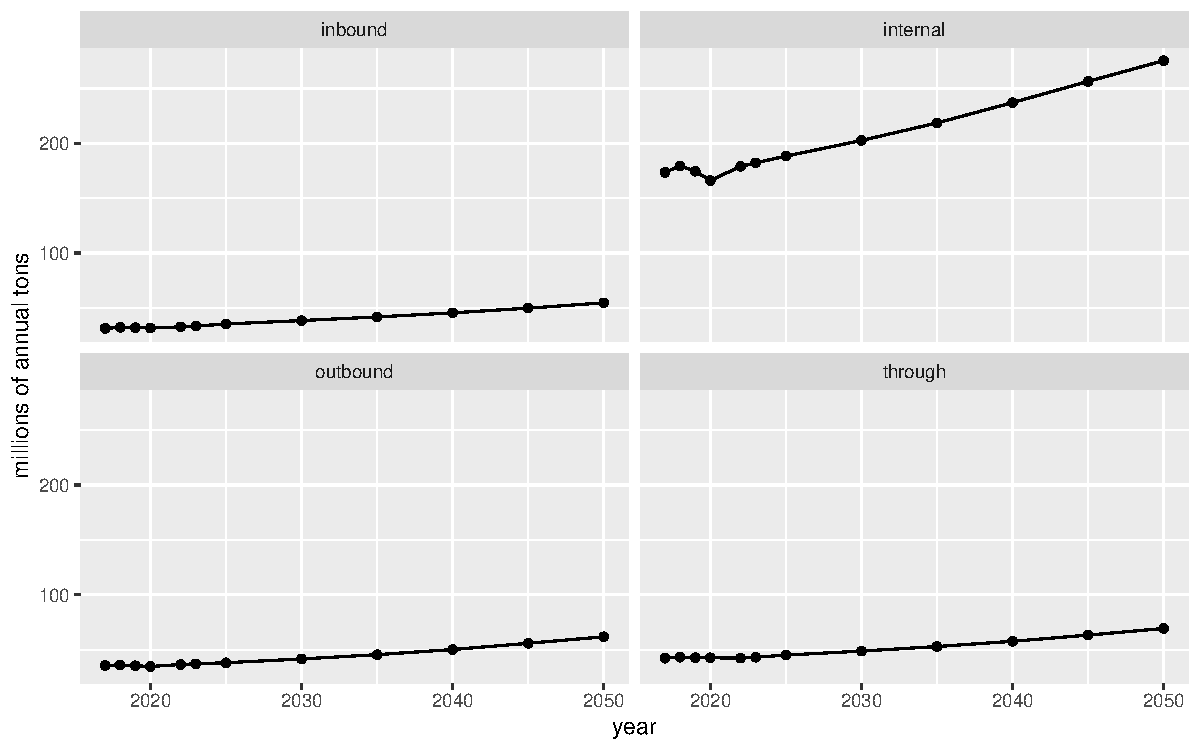
\includegraphics[width=5.5in]{figures/faf-growth-rates}
\caption{FAF Version 5.4 forecasted total tonnage within and through Oregon, 2020-2050}
\label{fig:faf-growth-rates}
\end{figure}

    \item Growth rates could be calculated ``on the fly'' from total production and consumption trends simulated in the AA or NED modules. Total production and consumption by industry would be appended to a temporary file during each simulation year. Growth rates from the previous year, or any number of years, could be calculated for each commodity group.\footnote{The AA module calculates production and consumption flows by transportable and non-transportable commodities. The former are indexed by the same SCTG codes used in the CT module. The latter includes land and structures, fixed assets, and other immovable factors of production.} This approach would maximize compatibility with the assumptions used in any given SWIM2 scenario and offer more geographic granularity than from a single fixed rate. However, this approach will be more difficult to implement because of the degree of message handling and data interchanges required. An interim solution might be to use exogenously calculated AA growth rates from several prior runs. This is functionally the same approach as the first option but informed by previous SWIM2 runs.
    \item Historical count data from the external zones can be used to construct a time series. The viability of this option depends upon a long series of robust counts (i.e., from automated traffic recorders) being available for each site. Using long-term growth rates from each external zone would allow the SWIM2 system to be sensitive to their differing growth rates. The downside of this approach is that the historical trends might not well depict the future, especially when testing scenarios that involve changes in infrastructure or route capacity. Using historical trends alone is viewed as a less defensible approach than one based upon FAF or AA trends.
\end{enumerate}

The current CT implementation includes the FAF growth rates shown in Table \ref{tab:faf-growth-rates}, with the values coded in a comma-separate value file. These values can easily be adjusted or replaced by the analyst using the other methods described above.

\begin{table}
\centering
\caption{FAF 5.4 compound annual growth rates (CAGR)}
\label{tab:faf-growth-rates}
\begin{tabular}{lrrr}
\hline
Direction & 2017 tonnage & 2050 tonnage & CAGR \\
\hline
Inbound & 31,317,751 & 54,603,564 & 0.0169886 \\
Internal & 173,552,636 & 275,398,131 & 0.0140904 \\
Outbound & 35,487,586 & 61,711,926 & 0.0169078 \\
Through & 42,201,856 & 69,307,990 & 0.0151468 \\
\hline
Total & 282,559,829 & 461,021,611 & 0.0149456 \\
\hline
\end{tabular}
\end{table}

\subsection{Local truck generation}

The data required to understand local CV travel behavior within Oregon comes from elsewhere. The use of synthetic or borrowed trip rates to estimate the total truck trips by purpose and type was assessed. The approach is quick to implement, and provides reasonability checks on estimates developed using more complex truck tour models. An older but widely used sketch planning tool \citep{beagan07} was used to develop these rates. The prototypical values for trip generation and distribution in the Manual were used in conjunction with Oregon time-of-day distributions in order to estimate truck trips by truck type and period of the day. The overall process is relatively simple, as shown in Figure \ref{fig:ct-trip-model}.

\begin{figure}[!b]
\centering
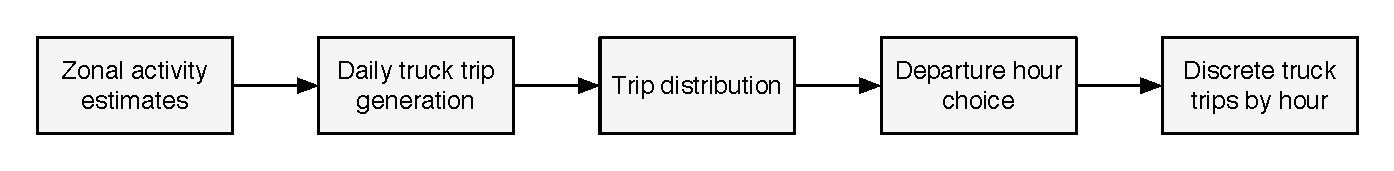
\includegraphics[width=6in]{figures/ct-trip-model.pdf}
\caption{Trip-based truck model structure}
\label{fig:ct-trip-model}
\end{figure}

An additive linear model is used to calculate trip ends within each zone. Five categories of firms and total households are used to calculate the trip ends $T_m$ for each truck type $m$:
\begin{equation}
T_m = \alpha_1 \thinspace AMC + \alpha_2 \thinspace COM + \alpha_3 \thinspace RET + \alpha_4 \thinspace OS + \alpha_5 \thinspace HH
\end{equation}

\noindent where the default parameters and those found to work best in Oregon are shown in Table \ref{tab:qrfm2-generation}. The firm categories used in the SWIM model (Table 2.3 on page 13 in the \textit{SWIM2.5 Model Delivery Report}) were each associated with one of the broad industry categories shown in the Table in order to calculate total truck trip ends at the zonal level. Note that this method assumes symmetry of flow on a daily basis, such that the calculated trip ends represent both total daily origins and destinations within each zone.

\begin{table}
\centering
\caption{Default and adjusted truck trip generation parameters}
\label{tab:qrfm2-generation}
\begin{threeparttable}
\begin{tabular}{llrrr|rrr}
\hline
 & & \multicolumn{3}{c|}{Default values\tnote{a}} & \multicolumn{3}{c}{Adjusted values\tnote{b}} \\
Parameter & Description & Light & Medium & Heavy & Medium & Heavy \\
\hline
AMC ($\alpha_1$) & Agriculture, mining, construction & 1.110 & 0.289 & 0.174 & 0.159 & 0.099 \\
\gray COM ($\alpha_2$) & Commercial firms\tnote{c} & 0.938 & 0.242 & 0.104 & 0.133 & 0.059 \\
RET ($\alpha_3$) & Retail trade & 0.888 & 0.253 & 0.065 & 0.140 & 0.040 \\
\gray OS ($\alpha_4$) & Office and services & 0.437 & 0.067 & 0.009 & 0.376 & 0.006 \\
HH ($\alpha_5$) & Households & 0.251 & 0.099 & 0.038 & 0.055 & 0.233 \\
\hline
\end{tabular}
\begin{tablenotes}
\footnotesize
\item[a] From \cite{beagan07}, Table 4.1
\item[b] Light trucks not included in the CT simulation or validation
\item[c] Includes manufacturing, transportation, communications, utilities, and wholesale firms
\end{tablenotes}
\end{threeparttable}
\end{table}

A doubly-constrained gravity model is specified for trip distribution, based upon adjusted values from the Seattle region. Simple exponential functions were used to estimates values of interzonal impedance $F_{ij}$ between $i$ and $j$ for two distance bands $d$ for each of the three truck types $m$:
\begin{equation}
F_{ijmd} = exp(\alpha + \beta C_{ij})
\end{equation}

\noindent An unspecified general cost $C_{ij}$ was used in the Seattle model, and the rates shown in Table \ref{tab:grfm2-distribution} were specified by the distance ranges shown. These average trip length values obtained using these rates in Oregon appeared reasonable, as shown in the Table. However, when assigned to the network the resulting origin-destination flows did not replicate observed truck counts across the state. Substituting the gravity model with the multivariate activity location choice model (\S\ref{sec:ct-activity-location}) produced better results, prompting an abandonment of the gravity model approach.

\begin{table}
\centering
\caption{Truck trip distribution parameters}
\label{tab:grfm2-distribution}
\begin{threeparttable}
\begin{tabular}{lrrcrrr}
\hline
& \multicolumn{3}{c}{Default values\tnote{a}} & \multicolumn{3}{c}{Average trip distance} \\
Truck type & $\alpha$ & $\beta$ & Distance & Published\tnote{a} & Simulated\tnote{c} & Difference \\
\hline
Light & 3.75 & -0.08 & $<$26 miles & 22.34 & 25.91 & 16.0\% \\
\gray Light & 2.1 & -0.005 & $\geq$26 miles & 22.34 & 25.91 & 16.0\% \\
Medium & 4.75 & -0.05 & $<$27 miles & 27.53 & 32.15 & 16.8\% \\
\gray Medium & 4.2 & -0.003 & $\geq$27 miles & 27.53 & 32.15 & 16.8\% \\
Heavy & 1 &  & $<$7.5 miles & 28.29 & 33.74 & 19.3\% \\
\gray Heavy & 5 & -0.009 & $\geq$7.5 miles & 28.29 & 33.74 & 19.3\% \\
\hline
\end{tabular}
\begin{tablenotes}
\footnotesize
\item[a] From \cite{beagan07}, \S4.1.2
\item[b] From \cite{beagan07}, Table 4.2
\item[c] Result based upon running model with delivered SWIM2 system
\end{tablenotes}
\end{threeparttable}
\end{table}

Individual trips are assigned a departure time, based on profiles constructed from data provided by Portland Metro for their truck model and preliminary data from the 2011 Commercial Vehicle Survey in Canada. The latter were thought to better depict intercity travel patterns better, while the former provides local context within which to assess their reasonability. The initial values performed well, but were iteratively adjusted to better match the temporal distributions found in truck counts used in model validation. The resulting trip departure time probabilities are shown in Figure \ref{fig:ct-trip-departure-times}. A departure time is sampled for each truck trip.

\begin{figure}
\centering
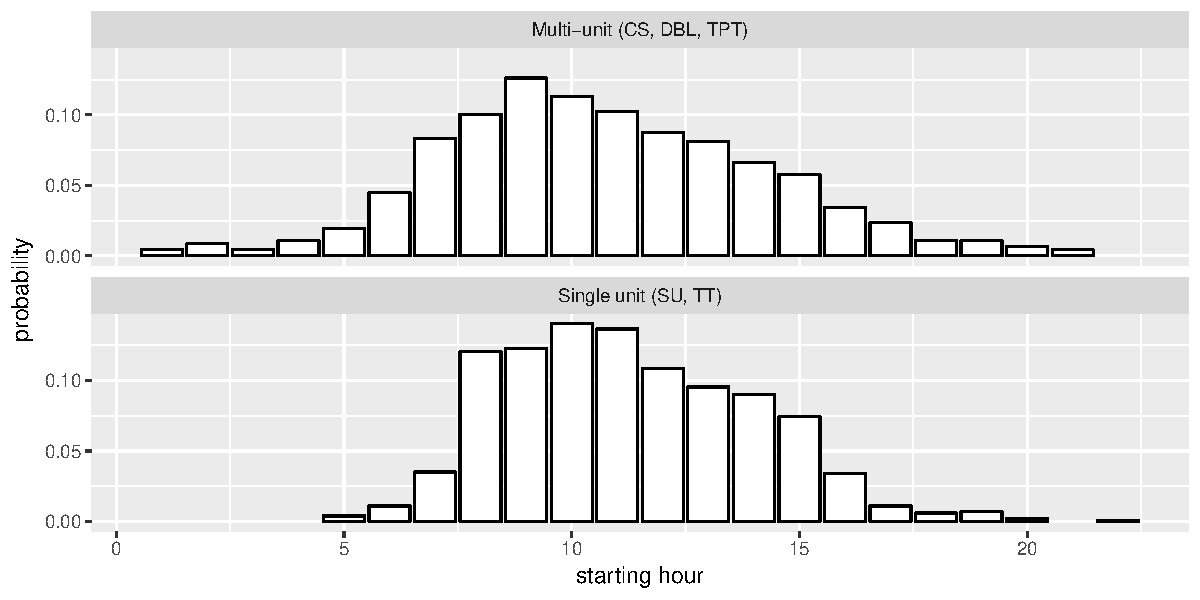
\includegraphics[width=6.25in]{figures/trip-start-hour.pdf}
\caption{Truck trip departure time profiles by truck types}
\label{fig:ct-trip-departure-times}
\end{figure}

%------------------------------------------------------------------------------
% Start local truck model description
\subsection{Truck tour generation}\label{sec:ct-tour-generation}

Firms within the modeled area trade with one another, as well as households. They also trade with firms and markets outside of the modeled area, either as imports or exports. Imports, whether domestic or foreign, are consumed in lieu of goods produced within the modeled area. Exports, on the other hand, are goods that are consumed outside of the modeled area, instead of within it. The AA module determines the levels of imports and exports based upon their prices in external markets versus those within Oregon and the halo.\footnote{See the last paragraph in \S6.1 (page 100) in the \textit{SWIM2.5 Model Delivery Report} for a general description. The underlying calculations are described in \S6.3.4 (page 110) in the same document.} As noted in \S\ref{sec:faf-integration}, the CT module uses the FAF data to define the distal trip ends (i.e., those outside of Oregon) for such flows, as well as the mode of transport. Because the FAF data in effect replaces the production-consumption flows from Oregon zones to and from the world markets the latter flows are discarded. 

What remains after imports and exports are handled are internal commodity flows within the model (i.e., flows with both trip ends within the modeled area). The FAF does include some flows between points within the modeled area, for the CFS includes gathers data on trips to destinations greater than 50 miles away.\footnote{The information on domestic truck flows in the FAF comes from the CFS. There are some truck flows less than 50 miles in the CFS (i.e., between FAF regions less than 50 miles apart), which are a combination of artifacts from the destination choice process used in the FAF and multi-stop truck tours in the CFS, where the first stop of a longer tour is less than 50 miles from the shipper. However, trips to single destinations less than 50 miles away are not retained in the CFS.} Thus, it might be asserted that the FAF includes all long-distance truck trips, where the latter is defined as those greater than 50 miles in length. Unfortunately, the sample size of the CFS has diminished over time as survey costs have kept pace with inflation, but its budget has not. Between the progressively smaller sample size, focus on longer trips, and sampling frame limited to mining, manufacturing, and some wholesale establishments we cannot assume that the FAF includes all truck trips longer than 50 miles. Thus, a process for handling local trips --- those less than 50 miles, as well as a smaller number of trips greater than 50 miles completed within the same business day --- are handled in this part of the CT modeling process.

Several methods for simulating local trips were evaluated:
\begin{enumerate}
\item The original CT module scaled the expanded CFS total value of shipments to the total value of transportable commodities generated by AA, for each commodity. These value was translated into total annual tonnage, which was then proportionally allocated to zones across the state that produced the commodity. There they were transformed into discrete shipments by mode of transport. Those carried by truck were sized using average payload weights and number of stops from data collected at Oregon weigh stations. This did not perform well, as the resulting estimates were biased towards long-distance flows in the CFS.
\item Data from establishment surveys from other places can be mined to determine the incidence of daily truck trips and tours by industry type, taking care to remove the long-distance trips (i.e., those that would overlap with the FAF) from the data. The data themselves are rarely available, but tabulations and summaries from several surveys have been published.
\item The production-consumption flows from AA for internal movements can be converted into shipments or truckload equivalents using asserted or surveyed average payload weights applicable to single-unit (SU) trucks. The latter are assumed to be predominately used for local CV tours, although data from truck intercept surveys such as the Vehicle Inventory and Use Survey (VIUS)\footnote{Microdata from the 2002 VIUS are available, and are almost singular source of data on the truck fleet in the USA. It was unfortunately discontinued due to budget cutbacks at the Census Bureau. The 2002 data are arguably close to the end of their utility for modeling, given how much the industry has changed over the past two decades.} and Canadian Commercial Vehicle Survey (CVS) can be used to estimate percentage of trips and tonnage by truck type.
\item A direct demand model can be asserted or estimated that equates AA employment or production levels, or production-consumption flows, with truck trips as a function of accessibility, distance, and other variables. A truck trip matrix constructed using origin-destination matrix estimation techniques, perhaps coupled with truck OD matrices from the Portland Metro truck model, can be used to help tune the model parameters.
\end{enumerate}

Maintaining consistency with AA was a major consideration in the choice of approaches, as were the resources available to test and evaluate alternative approaches. The first choice could easily be dismissed, based upon its mediocre performance in earlier versions of CT and exclusion of local trips from the CFS and FAF. Several establishment surveys were described in the literature, but few included detailed tabulations of key variables, alone or in combination. Considerable effort would have been required to work with individual researchers to obtain their data or have them carry out custom summaries of their data, which precluded further work in this area. It was felt that the third option, possibly in combination with the fourth, held the most promise for quick implementation.

The AA production-consumption matrices could not be mapped directly to truckload equivalents, due to the iterative proportional allocation of production to all possible destinations (consumption locations). Such an approach would yield a high number of truck trips with implausibly small volumes. Instead, the information in the PC flows were used in several stages to achieve the same effect. The overall structure of the resulting truck tour model is shown in Figure \ref{fig:ct-tour-model}.

\begin{figure}
\centering
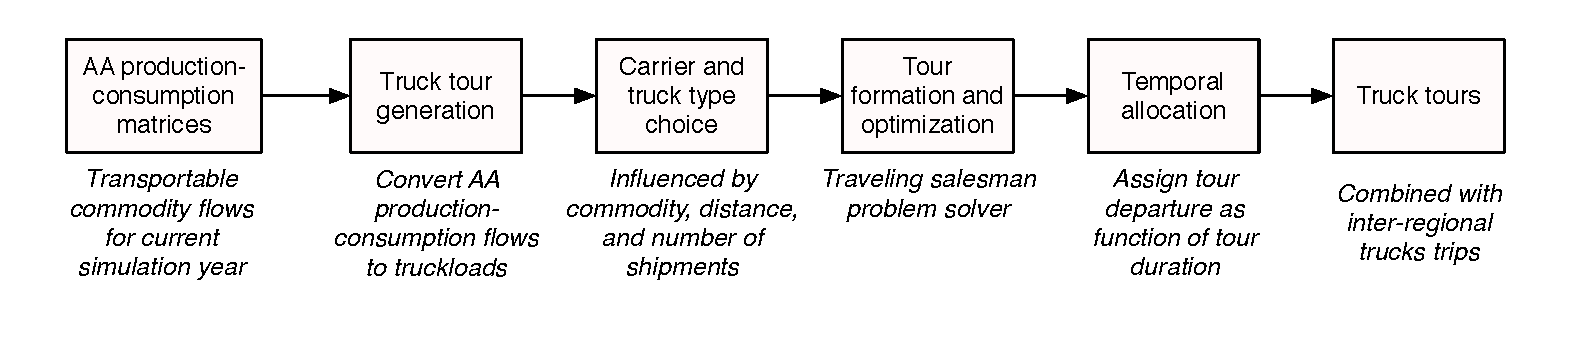
\includegraphics[width=6.25in, trim=0mm 8mm 0mm 0mm]{figures/ct-tour-model.pdf}
\caption{Structure of the CT truck tour microsimulation model}
\label{fig:ct-tour-model}
\end{figure}

%\subsection{Translation of PC flows into discrete shipments}

%The production-consumption flows $H$ of transportable commodity $k$ between production and consumption zones $p$ and $c$ are expressed in annual dollar terms. Thus, the level of production of $k$ in each zone can be obtained easily:
%\begin{equation}\label{eq:ct-zonal-production}
%H_{pk} = \sum_c H_{pck}
%\end{equation}

%If all zones had a large amount of production, as would be case if applying the model at the county or higher level, these annual dollar flows could be converted into annual shipments, which could be sampled at weekly and daily levels in the same manner as the FAF flow transformations described above. However, some zones have small amounts of annual production, which would translate into very small levels of weekly or daily activity. Thus, we can more easily create total annual shipments $V$ for commodity $k$ for the model area, and then allocate them to zone of production $p$ using the levels calculated in equation \ref{eq:ct-zonal-production} as weights in a probabilistic allocation.

%Average shipment sizes, calculated as a function of payload weight and number of stops by vehicle type, were derived by running the truckload equivalency process shown in Figure \ref{fig:ct-truckload-equivalents} for the range of tonnages shown in the data. The number of annual shipments $V$ for commodity $k$ for the modeled area is calculated as:
%\begin{equation}
%V_k = \left ( \sum_p H_{pk} / Z_k \right ) / G_k
%\end{equation}
%\noindent where:
%\begin{align*}
%V_k &= \text{Annual shipments of commodity $k$ generated within the modeled area} \\
%H_{pk} &= \text{Total production in zone $p$ of commodity $k$} \\
%Z_k &= \text{Ratio of value to tons for commodity $k$, derived from the FAF} \\
%G_k &= \text{Average shipment weight of commodity $k$}
%\end{align*}

%Each shipment can randomly be assigned to a week of the year, but allocation to day of the week is more complicated. Many firms consolidate shipments so that they can be carried out on one or a few days. Randomly assigning each shipment separately precludes such efficiency in freight movements. Many shippers do not have that luxury, of course, as customer demands dictate shipment schedules. Moreover, the picture gets even more complicated when for-hire trucks are considered, for further cost savings to the shipper might accrue if fewer pickups, each with more material, are scheduled during the week. Insight into these decisions could be added to establishment surveys, but information about them are not available now. We can assume that every day of the week is equally likely, and adjust parameters by industry sector based upon trip generation and special generator studies, as well as comparisons to overall traffic count levels. We found no appreciable difference between sectors, so used a simple factor of 0.272 as the threshold for selection in daily estimates.\footnote{If a random draw from the interval (0,1] was below the threshold (0.272 in this case) the shipment is selected for routing on the simulation day.} This was as much a data limitation as reflection of true behavior, for we ``backed into'' this estimate based upon successive runs of the model, comparing the aggregate traffic assignment statistics to observed flow patterns.

\subsection{Carrier and vehicle type choice}

All shipments from a given producer $p$ (origin) are first assigned a carrier type (private or for-hire) using a Monte Carlo process. The commodity-specific private carrier share has been summarized from the 2002 Vehicle Inventory and Use Survey (VIUS), and shown in Figure \ref{fig:ct-carrier-vehicle-types}(a). All shipments for a given production zone $p$ and commodity $k$ are assumed to have a consistent carrier type (i.e., private or for-hire). Since flows are organized by commodity and zone this has the effect of assuming that all shippers within a production zone $p$ make an identical carrier choice. This is a necessary assumption, for AA works in terms of employment and industry output rather than individual firms. Thus, it is not known whether employment within any given zone comes from a single large establishment or many smaller ones.

\begin{sidewaysfigure}
\centering
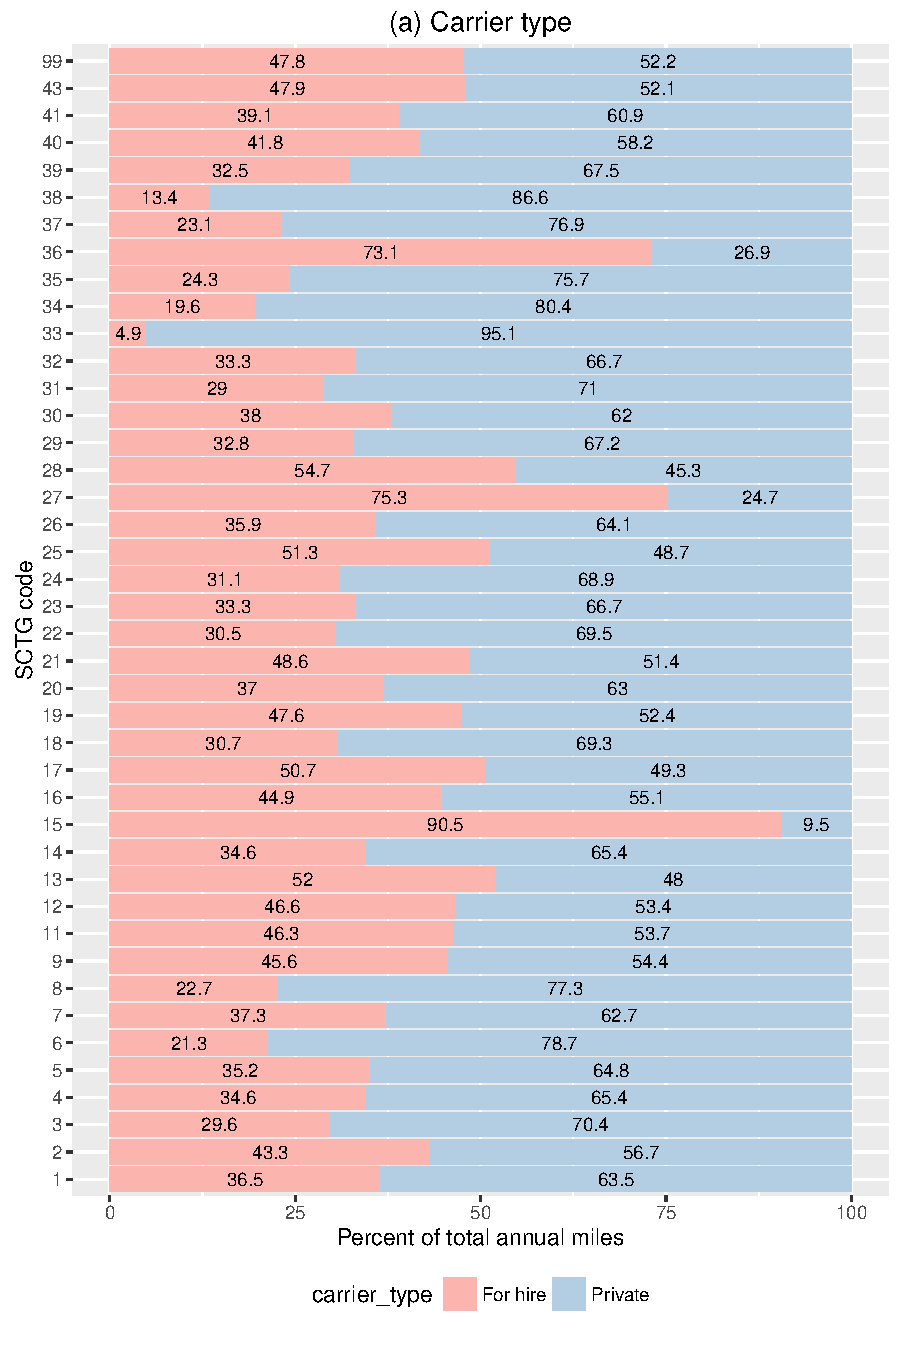
\includegraphics[scale=0.65]{figures/ct-carrier-types}
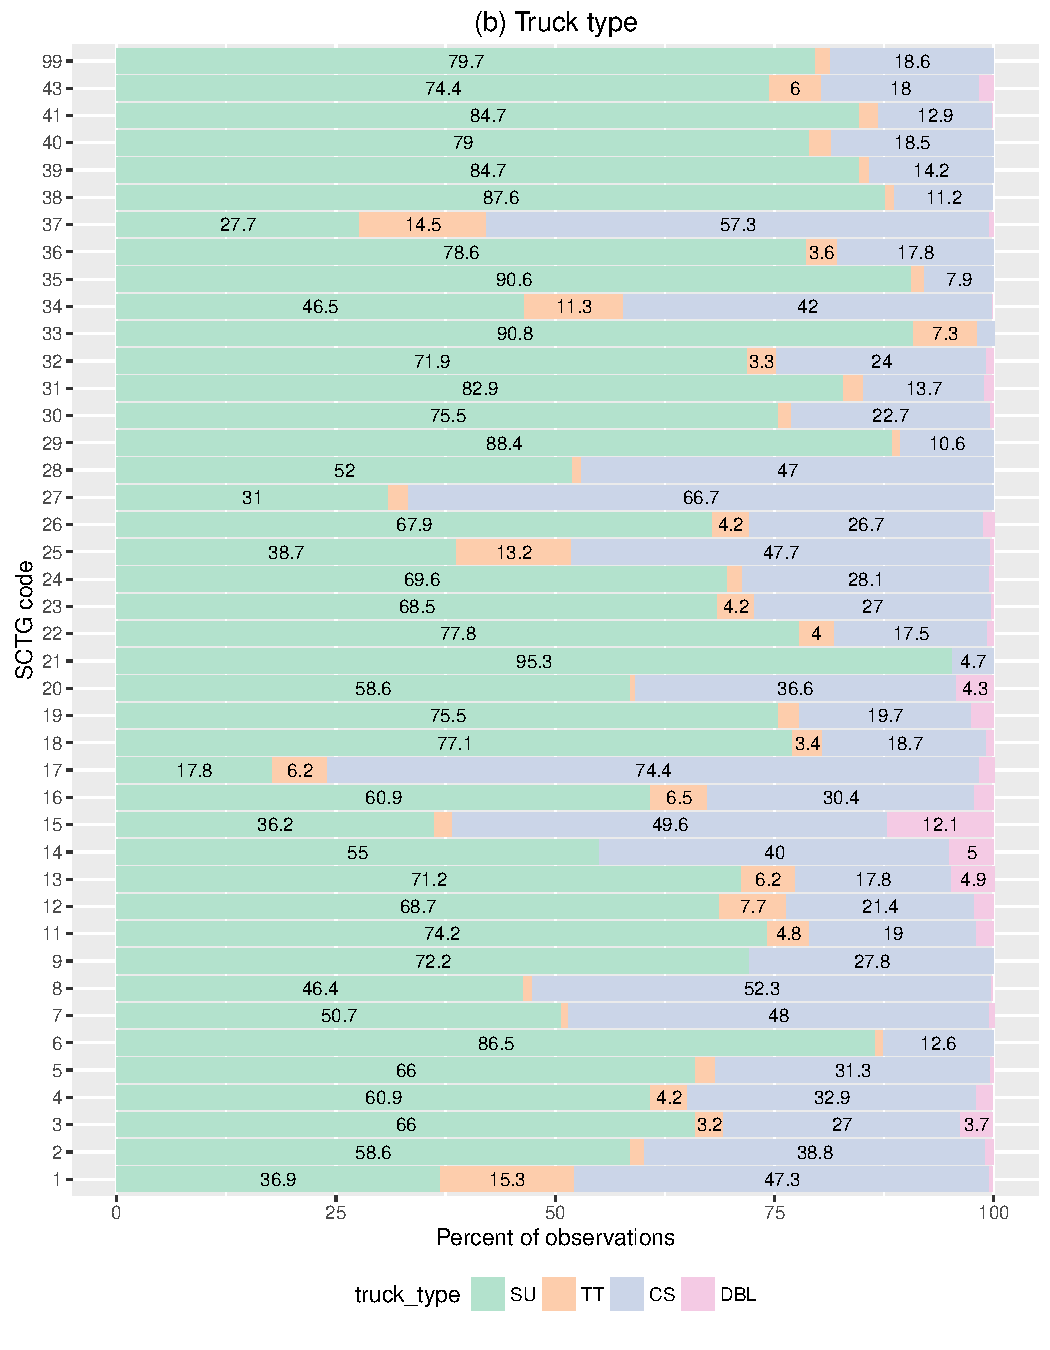
\includegraphics[scale=0.65]{figures/ct-vehicle-types}
\caption{VIUS carrier and vehicle type proportions by commodity}
\label{fig:ct-carrier-vehicle-types}
\end{sidewaysfigure}

A vehicle type is similarly selected, also based upon data from the VIUS. The percentages shown shown in Figure \ref{fig:ct-carrier-vehicle-types}(b). They are based upon the number of observations from the data, where the respondent reported that their range of operation was 200 miles or less. The number of observations were originally weighted by annual reported mileage, so that the percentages shown were exposure rather than incidence. It was thought that this would lead to better estimates of vehicles by type during network assignment. However, there was little difference between the weighted and unweighted outcomes when tabulating the percentages, while the former did slightly worse in assignment.

\subsection{Itinerary optimization}\label{sec:itinerary-optimization}

Truck itineraries can be assembled from the discrete shipments allocated to each production zone. The process for handling shipments on private trucks is simple. Shipments from each origin are loaded onto a truck until its average payload weight is reached, and then onto additional trucks as needed. The process is illustrated in Figure \ref{fig:ct-private-tour-formation}. The average payload weights from the CVS are used for this purpose, although the analyst can optionally define a different set of payload thresholds if desired.

\begin{figure}[!t]
\centering
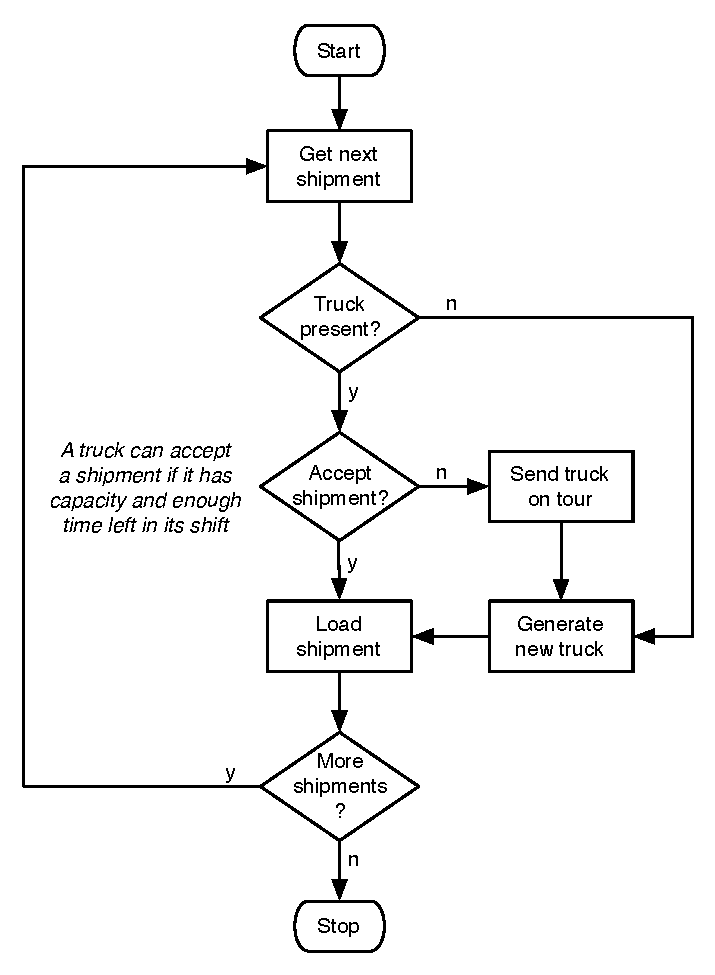
\includegraphics[scale=0.7]{figures/PrivateTrucks}
\caption{Process for creating private carrier truck tour itineraries}
\label{fig:ct-private-tour-formation}
\end{figure}

The process for handling for-hire carriers is more complex, in that they can accept shipments from more than one origin zone. At the first origin zone, for-hire trucks are loaded in the same manner described for private trucks. However, any for-hire truck not filled to capacity is tagged as ``available'' and placed in a list of available partially filled trucks. For all subsequent for-hire shipments, the closest truck within a user-specified range (currently 0.9 miles for SU trucks, and 2.5 miles for all others) with capacity greater than or equal to the shipment size is selected for carriage. Shipments are added to this truck until all for-hire shipments from the origin are accommodated or until the vehicle reaches capacity. If the vehicle reaches capacity the search for another ``available'' vehicle is repeated. In the event that an available truck with adequate capacity is not found within the specified search radius a new empty for-hire truck is created, filled with the shipment(s), and placed in the available if appropriate. The process is shown in Figure \ref{fig:ct-forhire-tour-formation}.

\begin{figure}[!b]
\centering
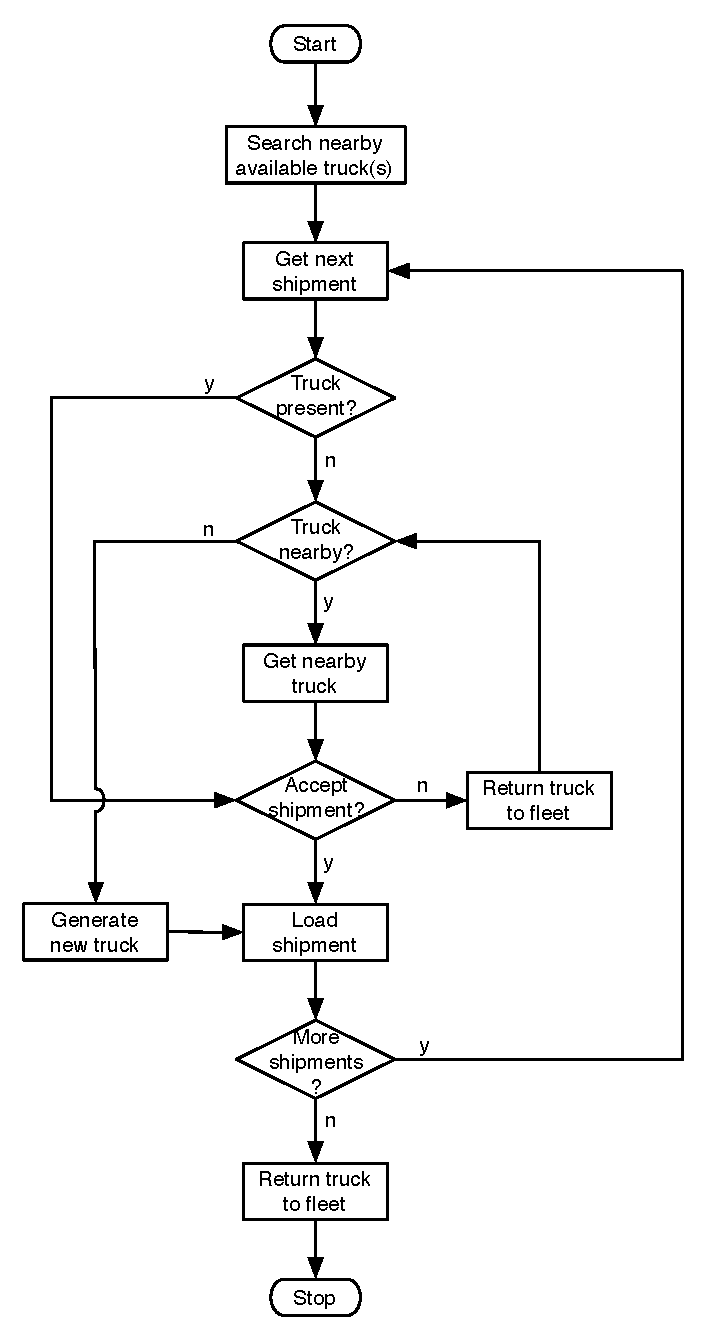
\includegraphics[scale=0.7]{figures/ForHireTrucks}
\caption{Process for creating for-hire truck tour itineraries}
\label{fig:ct-forhire-tour-formation}
\end{figure}

The model also imposes an additional constraint on the for-hire vehicle selection. Each vehicle is only allowed to handle a maximum number of pickups. The result is that many do not fill to capacity before becoming ineligible to add additional shipments. This is a common occurrence in the LTL industry, making this plausible behavior to add to the model.

Before a shipment is added to a vehicle, the vehicle must not only be able to hold the total weight of the shipment(s), but also must not exceed the driver shift duration limit. A vehicle's travel time is updated with each shipment to include the travel time to the new shipment, the dwell time of the pickup activity, as well as the resulting travel time to the final destination. The travel times are estimated using the congested off-peak period travel time matrices for the previous model period.

Once all shipments are assigned to vehicles the itineraries are optimized to minimize total travel time on the tour. The shipment list is first sorted by vehicle identifier (i.e., a specific truck itinerary). Each vehicle carries one or more shipments, each possibly having a different destination. Each destination is coded as a stop in a tour that will serve all destinations for that specific vehicle in sequence. For-hire trucks that pick up loads from more than one zone will also have stops coded for the additional origins. A classical traveling salesman problem (TSP) algorithm is used to generate the solution. It returns all for-hire vehicles to the origin after the last stop, partially solving the problem of empty backhauls. More complex routing methods were investigated, such as the vehicle routing problem with backhauls, but did not appear to offer significant advantages over the TSP solution.

\subsection{Activity location choice}\label{sec:ct-activity-location}

Most urban truck tours include multiple stops, some involving a dozen or more places. Data on such patterns are still hard to come by, as commercial vehicle surveys with complete diaries are still rare. Such surveys have not been conducted in Oregon, forcing a reliance on tour pattern data collected elsewhere. \cite{holguinveras05} published one of the first comprehensive analyses of urban truck tour patterns, based upon data from Denver. Their findings were used to validate the initial version of CT, along with unpublished data from Houston and Ohio. The Denver results do not include information about the spatial aspects of tour formation, although such could be inferred from the other sources available to the team. 

The variability of these patterns was always a question, which research by \cite{figliozzi07a} helped frame. He followed 500 trucks in Sydney for a period of six months. While tour structure remained constant for most respondents he found that few trucks repeated the same route twice within those six months. \cite{sharman11} found the same pattern when looking at GPS traces from long-haul trucking. We found the same to be true when analyzing GPS tracking data for 32,498 trucks from 981 firms operating in Southern Ontario in 2014-15. This makes the use of traditional activity location choice (ALC) models challenging in the absence of consistency in choices. The choice is further complicated by the absence of a primary tour destination (e.g., workplace, school location), which helps constrain ALC models of person travel. Had GPS tracking data been available in Oregon it might have been possible to fuse them with business location data to develop traditional ALC models. In their absence we tested two different approaches:
\begin{itemize}
\item It is assumed that the value of goods and services follow the same patterns as the trade (monetary flows) between firms and households, as revealed in the input-output (IO) matrices produced by AA (\S6.5.2 in the \textit{SWIM2.5 Model Delivery Report}). That is, the output of each firm in sector $a$ is consumed in different fixed proportions by other firms in $a$, as well as firms in all other sectors. Thus, the total value of trade between industries in the IO matrix defines a set of proportions that can be sampled from in order to choose the type of firm most likely to produce of consume it. We can combine these coefficients with a distance decay function in order to constrain the ALC to the firms most likely to trade with any given firm. This approach maximizes consistency with the results produced by the AA module (\S6.6 in the \textit{SWIM2.5 Model Delivery Report}).
\item The relative attractiveness of each zones can be more simply computed as its share of socioeconomic activity, at a more aggregate level of activity that varies by tour purpose. As with the previous approach, the attractiveness of a zone is inversely proportional to its distance from the current stop location. \cite{hunt07} use a variant of this approach in their commercial vehicle model in Calgary, an adaptation of which is also used in the Ohio statewide model. 
\end{itemize}

We found that the two approaches performed almost about the same in Oregon. The second was harder to implement because of its logit formulation, for parameter estimates derived elsewhere did not replicate Oregon conditions well. Moreover, the model calculates the number and location of stops on the fly, but difficult to tune to match the target values while remaining within the range of parameter estimates used elsewhere. The best fit, in terms of overall model replication of observed truck flows by type (local versus long-distance) and truck type, was obtained using a hybrid approach. The number of stops per tour were sampled from observed distributions by tour purpose and truck type. For each stop we can likewise sample an ideal trip length $\delta$ from the observed trip length distribution. Interzonal distance was used in this case, as most of the target data measured spatial separation that way. However, travel time or generalized cost could also have been used. The utility of each destination $j$ from the current location $c$ is calculated as:

\begin{equation}
U_j = \alpha {1 \over {| d_{cj}-\delta} |} \times \beta {A_j \over \sum A_j}
\end{equation}

\noindent $\alpha$ and $\beta$ are weights that can be used for each term, while $d_{cj}$ is the distance between $c$ and $j$ and $A_j$ are the attractions. The inverse is used in the first term to rank those destinations closest to the ideal distance higher than destinations further from it. Values of $\alpha = 11.0$ and $\beta = 0.2$ were found to produce the best results. 

It was assumed that most tours are closed, requiring the truck to return to the tour origin as its last stop. However, the heuristic described above chooses each stop location independently. Previous stops are excluded, but otherwise the stop location search does not consider whether it is moving closer to the tour origin, or away from it. \cite{hunt07} ``bend'' the trip back towards the origin with successively higher weights in their model, whereas most others use a traveling salesman problem (TSP) solver to order the stops. A simpler solution was devised in this case, where only a subset of eligible destinations closer to it were considered. Once the values for the ideal trip lengths $\delta_k$ are chosen the furthest distance $W$ each destination $j$ can be from the tour origin $h$ is computed as:

\begin{equation}\label{eq:search-diameter}
W = {\bar \delta_k} \sqrt{n}
\end{equation}

\noindent where $n$ is the number of stops in the simulated tour. Destinations further away than $W$ were excluded from the list of alternatives. The use of this constraint prevented the case where the final trip (tour segment) was much longer than the ideal distance (or in many cases, substantially longer than the average trip length). The solution can optionally be further refined using a TSP solver, although in calibration it was found to provide only a small improvement in solution quality. The model constrained in this manner (i.e., using equation \ref{eq:search-diameter}, but not TSP solution) closely replicated the observed trip length frequencies, as shown in Figure \ref{fig:ct-observed-trip-lengths}. 

\begin{figure}
\centering
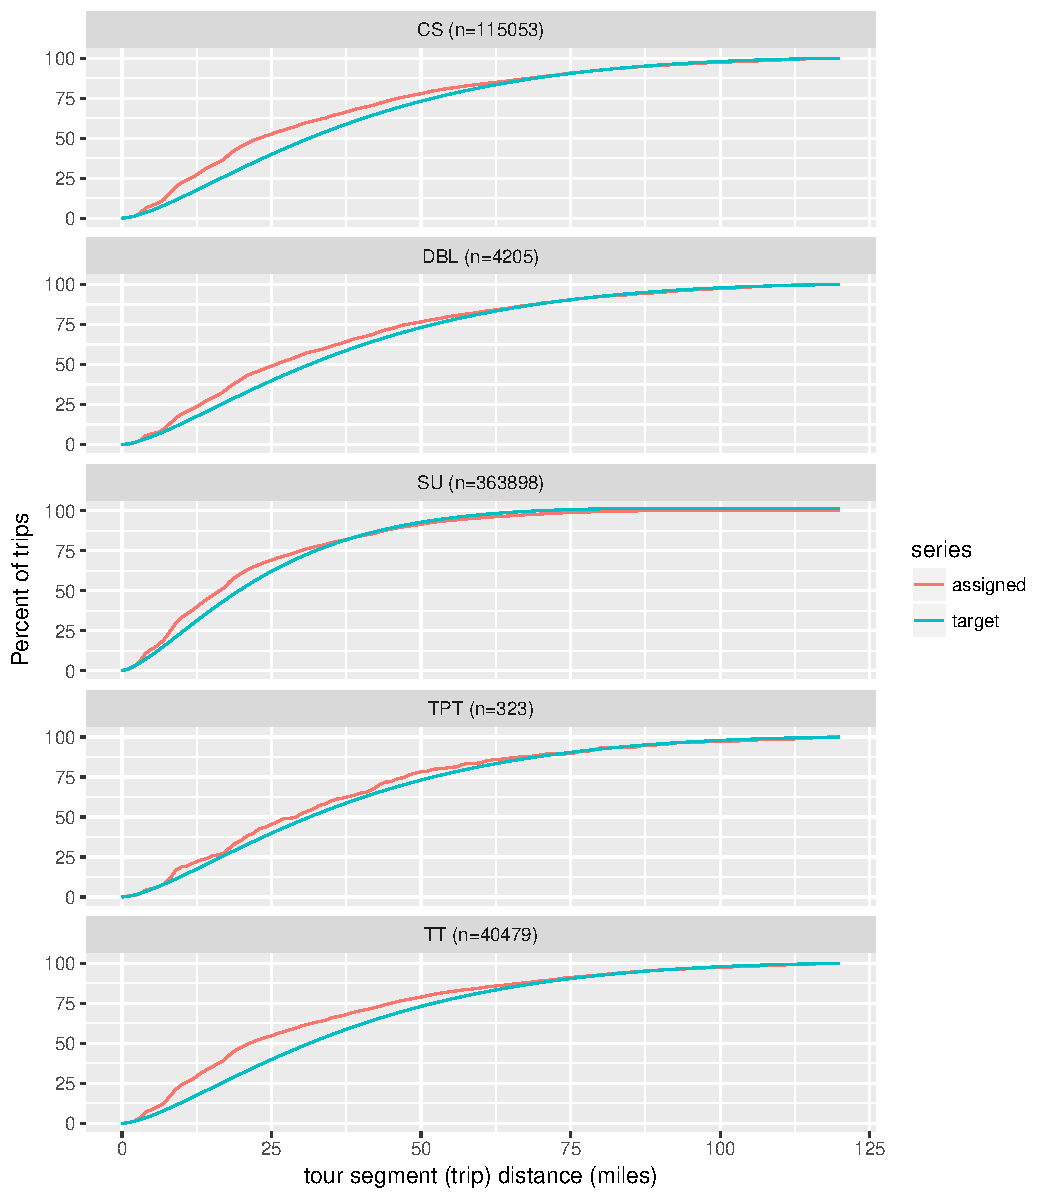
\includegraphics[scale=0.95]{figures/trip-length-comparisons.pdf}
\caption{Observed versus simulated cumulative trip length frequency distributions by truck type}
\label{fig:ct-observed-trip-lengths}
\end{figure}

\subsection{Tour start time choice}

The final step in truck tour generation is the assignment of a tour start time (first departure). The start time is randomly assigned to each tour in the database. However, how it is assigned differs based upon the type of tour:
\begin{itemize}
\item For all internal trips, and FAF inter-regional trips with domestic origin in Oregon, the starting time is drawn from an observed distribution from a 2004 truck survey conducted in Houston. They classified vehicles by three types, and the relationship between tour duration --- which is already known --- and tour starting time is shown in Figure \ref{fig:ct-temporal-points}. A Loess fit is shown, which is almost linear, showing the expected finding that longer tours start earlier in the day, with a heavy concentration of tours starting early in the morning. The distribution of starting times can be more clearly seen in Figure \ref{fig:ct-temporal-distributions}. Such a distribution is generated for each hour of tour duration, and starting time is randomly sampled from it. 
\item For inbound FAF inter-regional trips (i.e., those with origin outside of Oregon) the hours are reversed, and then sampled as for internal trips. This ensures that they will follow the distributions shown in Figure \ref{fig:ct-temporal-distributions} during the last hours of their trip, which are those spent on Oregon roadways. The itinerary is then reversed again to return it into the proper order of stops.
\item For through FAF inter-regional trips the departure time is drawn randomly from the 24 hours of the day, for we have no data on arrivals at the Oregon border.
\end{itemize}

\begin{figure}
\centering
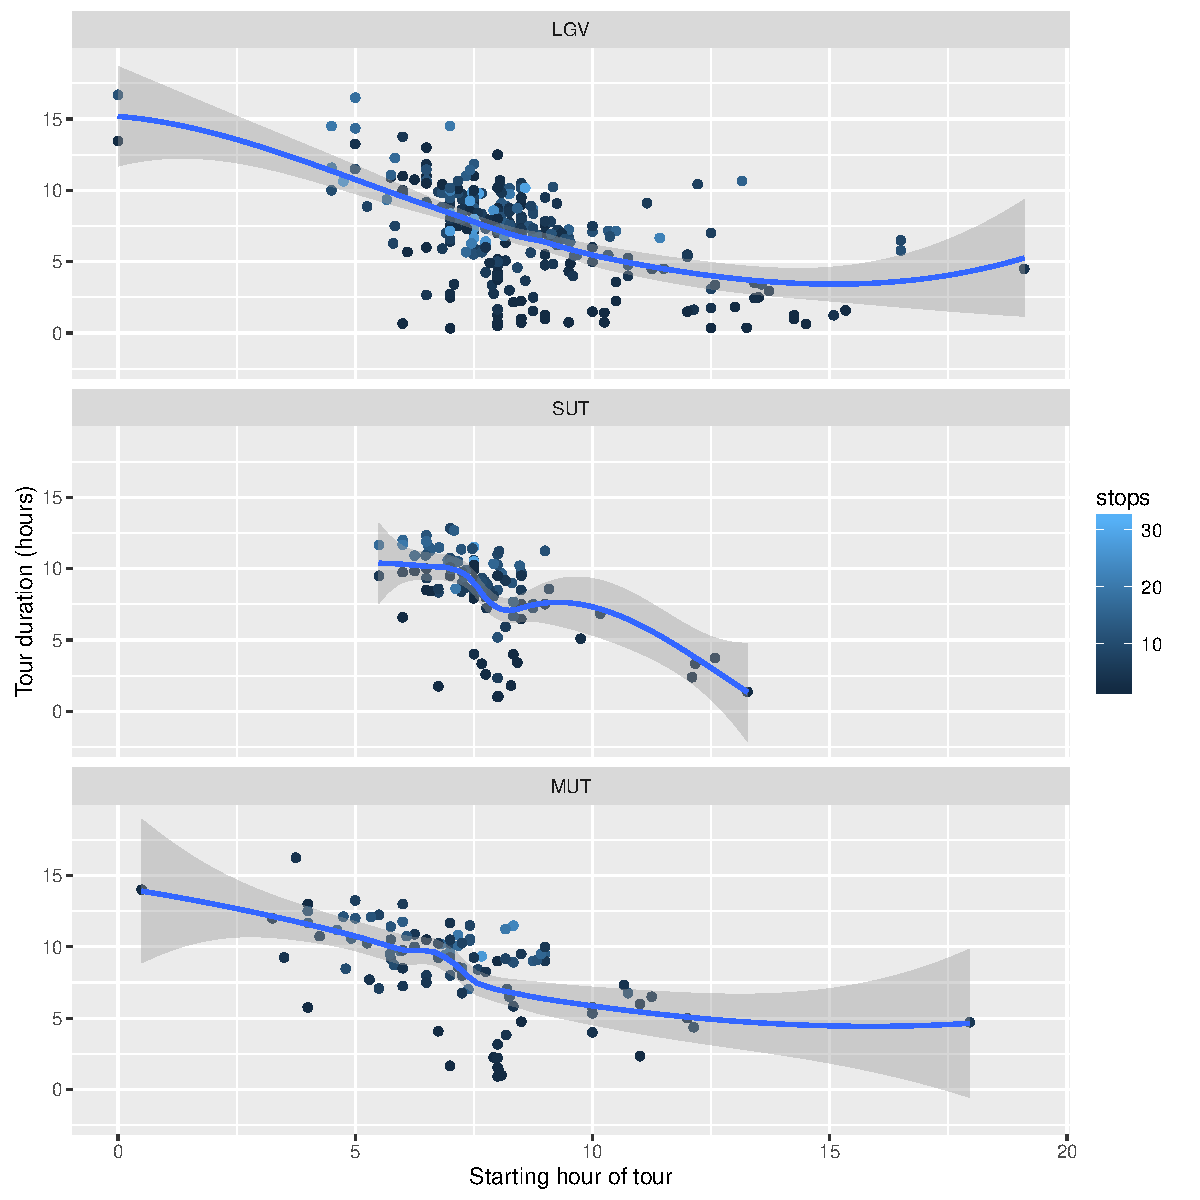
\includegraphics[scale=0.65]{figures/tours-temporal-distribution1.pdf}
\caption{Relationship between truck tour duration and starting time}
\label{fig:ct-temporal-points}
\end{figure}

\begin{figure}
\centering
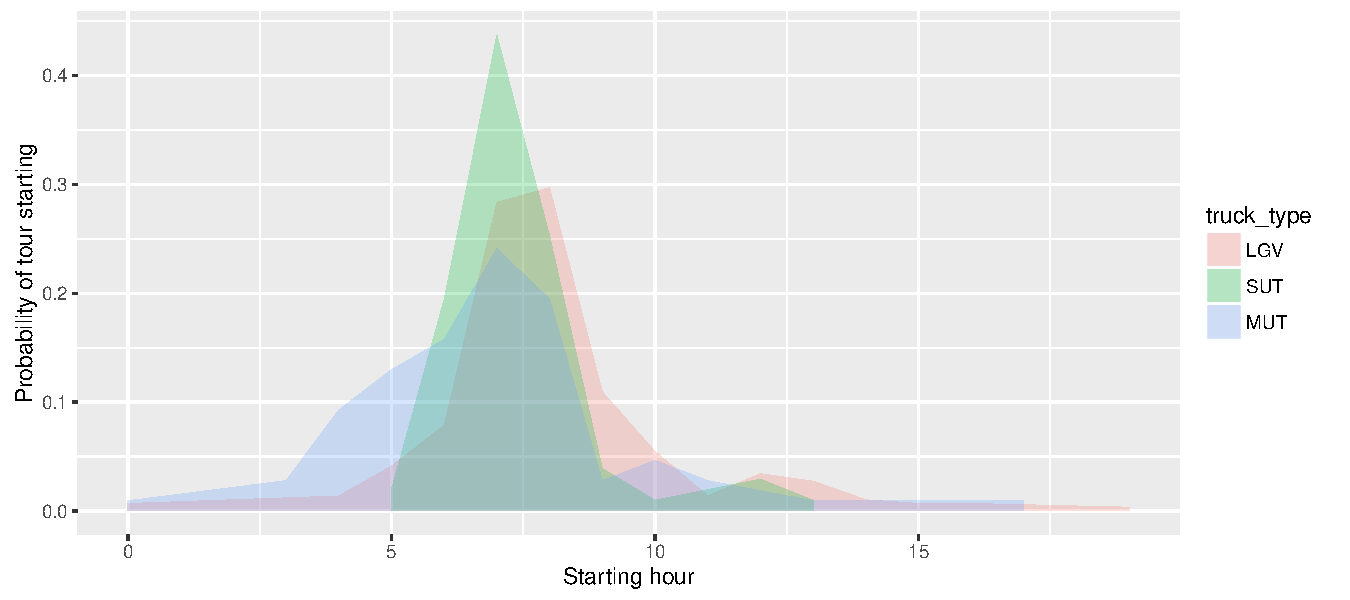
\includegraphics[scale=0.65]{figures/tours-temporal-distribution2.pdf}
\caption{Tour starting hour by truck type}
\label{fig:ct-temporal-distributions}
\end{figure}

The resulting distributions probably better describe urban rather than rural patterns. However, most truck tours begin or operate mostly within urban areas, making this an acceptable assumption for the entire modeled area. Note that the distributions derived using this process are not the same hourly distributions of truck traffic obtained from traffic counts, nor can the latter be substituted for the former. One depicts when tours begin, while the other reveals their cumulative presence on the network during the tours. 

After the starting time is selected the departure times for subsequent legs in the itinerary (trips) are obtained by adding the dwell and travel times for that leg to the previous departure time. The individual trips in the tour list are converted into origin-destination flows at the alpha zone level by truck type. These trip tables are then assigned to the network concurrently with the person travel flows generated by the PT module.

% End of truck tours sections
%--------------------------------------------------------------------------

\section{Software implementation}

The original CT module was written as a monolithic application in the Java programming language, following the same general pattern as the other SWIM modules. The current version of the model is written in the R statistical language, which is widely used at the Oregon DOT. It is implemented in the \verb|tlumip/swimctr| package, which bundles the code and default configuration items into a single package that can be easily installed or updated. Many of the models in the CT module are implemented as parallel processes using the doParallel package\footnote{\url{https://cran.r-project.org/web/packages/doParallel/vignettes/gettingstartedParallel.pdf}}.

An asymmetric TSP solver in R developed by \cite{hahsler07} is currently used by the CT module.\footnote{\url{https://github.com/mhahsler/TSP}} It replaces the Concorde TSP solver\footnote{\url{http://www.math.uwaterloo.ca/tsp/concorde.html}} used in previous versions of CT. 

The CT module reads the outputs produced by other modules, as well as its own configuration and parameter files (see \S\ref{sec:ct-input-output}) in compressed matrix or comma-separate value (CSV) formats. Its output is a list of discrete truck trips and aggregate flows by commodity and mode, both in CSV format. The CT modules typically runs in 10--20 minutes, depending upon the number of cores and speed of the processors. 

\section{Inputs and outputs}\label{sec:ct-input-output}

A number of runtime properties are required to run CT, as shown in Table \ref{tab:ct-module-inputs}. Several of the properties are inherited from the SWIM runtime parameters, which are read by CT to extract system-wide information such as the root directory when files are found and the simulation year. A number of observed or asserted distributions are required for both the inter-regional and truck tour components. Which component uses these inputs are unambiguous, for the property name is preceded by the component that requires it (i.e., ``faf'' for inter-regional, ``ct'' for urban truck tours).

\begin{sidewaystable} 
\centering
\caption{CT module inputs}\label{tab:ct-module-inputs}
\begin{tabular}{l L{4.75in} l}
\hline
Property & Description & Default value \\
\hline
ct.alpha2beta & Path to zonal equivalencies file & None \\
\gray ct.cluster.logfile & Name of CT cluster log file when running in parallel mode & None \\
ct.codePath & Path to where the CT package code exists & None \\
\gray ct.destination.utilities & Scaling factors for size terms in stop location choice model & ct\_destination\_utilities.csv \\
ct.distance.skims & Interzonal distances on the shortest travel time path & None \\
\gray ct.external.constraints & Observed and projected truck flows at SWIM2 external zones & ct\_external\_constraints.csv) \\
ct.filePath & Path to output folder & None \\
\gray ct.generation.probabilities & Constraints for tour generation in trips/employee & ct\_local\_generation\_probabilities.csv \\
ct.intermodal.connectors & Zones where freight transfers between truck and marine or air cargo ports within each FAF region within SWIM2 modeled area & ct\_intermodal\_connectors.csv \\
\gray ct.logfile & Name for CT log file & None \\
ct.maximum.resampling.attempts & Integer value that controls the  number of times the tour generation sampling will repeat if it does not finish with same number of trips calculated in aggregate for the entire study area & 100.0 \\
\gray ct.maximum.resampling.threshold & Floating point number defining how close the simulation must match aggregate number of trips for the entire modeled area & 1.0 \\
ct.outdir & Path to scenario output folder & None \\
\gray ct.properties.folder & Path to input parameters & None \\
ct.property & Path to `ct.properties` file & None \\
\gray ct.rcode & R script that runs the CT model & None \\
ct.sector.equivalencies & Mapping of AA sectors to CT industry categories & ct\_sector\_categories.csv \\
\gray ct.synthetic.population & Synthetic households file for the current SWIM2 simulation year & SynPop\_Taz\_Summary.csv \\
ct.temporal.factors & Hour of day distributions by truck type & ct\_truck\_temporal\_distributions.csv \\
\gray ct.travel.time.skims & Interzonal travel times on the least cost path & None \\
ct.trip.length.targets & Trip length distributions by truck type & ct\_trip\_length\_targets.csv \\
\gray cvs.payload.distributions & Distribution of payload weights by truck type & cvs\_payload\_weight\_distributions.csv \\
\gray faf.flow.data & Preprocessed FAF regional database for SWIM2 modeled area & prebuilt\_faf\_multiyear.csv.xz \\
faf.truck.allocation.factors & Proportions of long distance trucks by vehicle type & faf4\_truck\_allocation\_factors.csv \\
\gray pecas.makeuse & AA make and use flows for the current simulation year & MakeUse.csv \\
pecas.zonal.employment & AA zonal employment estimates by sector & Employment.csv \\
\hline
\end{tabular}
\end{sidewaystable}


The long-distance and local truck tour segments (i.e., trips) are combined into a single table for network assignment. The resulting table resembles what a daily travel diary for all trucks operating within Oregon would look like if such data could be collected. In addition, the CT module optionally saves a number of intermediate files that can be used for data mining or software testing, if desired. The typical files produced by the model are shown in Table \ref{tab:ct-module-outputs}, and the fields in the final trip list in Table \ref{tab:ct-triplist-layout}. 

\begin{table}  % 7 46
\centering
\caption{CT module outputs}\label{tab:ct-module-outputs}
\begin{threeparttable}
\begin{tabular}{L{3.3in} L{1.7in} l}
\hline
Data element & File(s) & Users \\
\hline
Zonal activity estimates & zonal\_data.csv & Diagnostics \\
\gray Daily local truck trip origins\tnote{a} & daily\_truck\_origins.csv & Diagnostics \\
Hourly local truck trips$^a$ & hourly\_truck\_trips.csv & Diagnostics \\
\gray Daily local truck tours\tnote{b} & daily\_truck\_tours.csv & Diagnostics \\
Daily local truck tour stops$^b$ & daily\_truck\_stops.csv & Diagnostics \\
\gray Daily local truck tour stops with activity locations$^b$ & located\_truck\_stops.csv & Diagnostics \\
Annual FAF truckload equivalents & annual\_faf\_trucks.csv & Diagnostics \\
\gray Daily FAF truck trips & daily\_faf\_trucks.csv & Diagnostics \\
Daily FAF truck trips with activity locations & located\_faf\_trucks.csv & Diagnostics \\
\gray Hourly FAF and local truck trips & combined\_truck\_trips.csv & CT, VISUM \\
\hline
\end{tabular}
\begin{tablenotes}
\footnotesize
\item[a] Files typically generated when running the trip-based framework
\item[b] Files typically generated when running the tour-based framework
\end{tablenotes}
\end{threeparttable}
\end{table}


\begin{sidewaystable}
\centering
\caption{CT trip list record format}\label{tab:ct-triplist-layout}
\begin{threeparttable}
\begin{tabular}{llcl}
\hline
Field & Description & Type & Values \\
\hline
truckID & Unique identifier for each truck & Integer & 1:number of simulated trucks \\
\gray origin & Origin alpha zone number & Integer & All valid alpha zone identifiers \\
destination & Destination alpha zone & Integer & All valid alpha zone identifiers \\
\gray tripStartTime & Trip departure time & Integer & hour and minute in 24-hour clock (hhmm) \\
tourMode & Type of truck tour & String & Internal, Inbound, Outbound, Through \\
\gray tripMode & Status of the truck contents & String & loaded, empty \\
truckType & Truck type used in the model\tnote{a} & String & SU, TT, CS, DBL, TPT \\
\gray sctg2 & Standard Classification of Transported Goods code\tnote{b} & Integer & 1-43, NA for trucks not carrying goods \\
value & Value of freight carried & Numeric & NA for service and other non-freight tours \\
\gray tons & Tonnage of freight carried & Numeric & NA for service and other non-freight tours \\
travelTime & Travel time in minutes & Numeric & Currently coded NA for FAF trips\tnote{c} \\
\gray distance & Trip distance in miles & Numeric & Currently coded NA for FAF trips$^c$ \\
dataset & Model that produced flow & String & faf, ct \\
\hline
\end{tabular}
\begin{tablenotes}
\footnotesize
\item[a] Truck types defined in Table \ref{tab:faf-truck-configuration}
\item[b] Coded to freight carried on previous tour segment (trip) when tripMode is empty
\item[c] The lack of external network precludes skimming of inter-regional freight flows
\end{tablenotes}
\end{threeparttable}
\end{sidewaystable}


\section{Calibration targets and outcomes}

The CT module is a microsimulation framework that employs a variety of modeling approaches, ranging from traditional deterministic models to Monte Carlo simulation (MCS). A variety of data were borrowed from elsewhere were used to develop the models. Most of these data were observed patterns reported in the literature, the underlying data for which are unavailable, or sensor data that lack information about the traveler, trip, or associated firms or land use. Thus, there were few opportunities to formally estimate model structures or parameters. Moreover, the underlying variances associated with the modeled behavior are known to be quite large (\S\ref{sec:ct-large-variances}), rendering traditionally estimated and calibrated deterministic models less than ideal for replicating them. The lack of suitable revealed or stated preference survey data for estimation further reduces the applicability of traditional modeling frameworks. As a result, the development of the CT module relied from a formidable data fusion and reconciliation effort. The resulting patterns and relationships were compared to limited observed data in order to validate it.

Given the data and conceptual limitations the CT module was formulated as a hybrid approach, fusing static aggregate FAF forecasts allocated to the level of detail required by SWIM2 with a microsimulation of truck tours. Calibration or validation of the former is neither possible nor practical, for the flows are assumed robust, with no ability to modify them except through ad hoc changes. While there are some behavioral models in the latter the majority were MCS outcomes. Thus, we can compare aggregate outcomes to observed data, the results of which are described in this section. We can categorize the tests we completed in two broad categories:
\begin{itemize}
\item \textit{In-scope comparisons:} When using MCS we routinely checked that the model closely reproduced target distributions, typically achieving a coincidence ratio\footnote{The coincidence ratio is the intersection of two normalized distributions divided by the union, as described in \cite{cambridge10}, \S6.2.2. Otherwise identical distributions have some stochastic noise, meaning that the ratio will approach unity, but never achieve it.} of 0.95 or better. Exact replication was typically not feasible due to the stochastic nature of MCS and random effects in the model (e.g., effect of using different random number seeds). 
\item \textit{Out-of-scope comparisons:} Comparisons of the outcomes were made to aggregate data not used in model development or application. In this case simulated truck flows were compared to observed flows by vehicle type and period of the day.
\end{itemize}

The in-scope tests are conducted as part of model runs, and not reported here. The CT module's ability to pass those tests were verified before the final model testing began. The validation is therefore restricted to the out-of-scope testing. ODOT has assembled truck count data from 2017 from 175 automatic traffic recorder locations across the state. Data on total flows were available for all years, but vehicle classification count data were sometimes only available every second or third year. Thus, data for two years on either side of the calibration year of 2020 were used in these analyses. In most applications the different truck classes shown in Table \ref{tab:faf-truck-configuration} are combined into a single truck category for network assignment, and the same aggregation is used in project appraisal. While there are considerable differences in trip characteristics by truck type, as described in previous sections, their assignment is compared in aggregate to observed flows. 

Both graphical and tabular comparisons were used to evaluate the validity of the CT module. Comparisons of simulated versus observed truck flows by ODOT region are shown in Figure \ref{fig:ct-link-scattergram}. The points would ideally line up on the diagonal (i.e., the dashed line defined by points where the observed and simulated volumes are equal). In some cases the results appear worse than in reality. The patterns look reasonable with only a small number of apparent outliers. Note that all counts were included in the validation without trimming outliers.

\begin{figure}
\centering
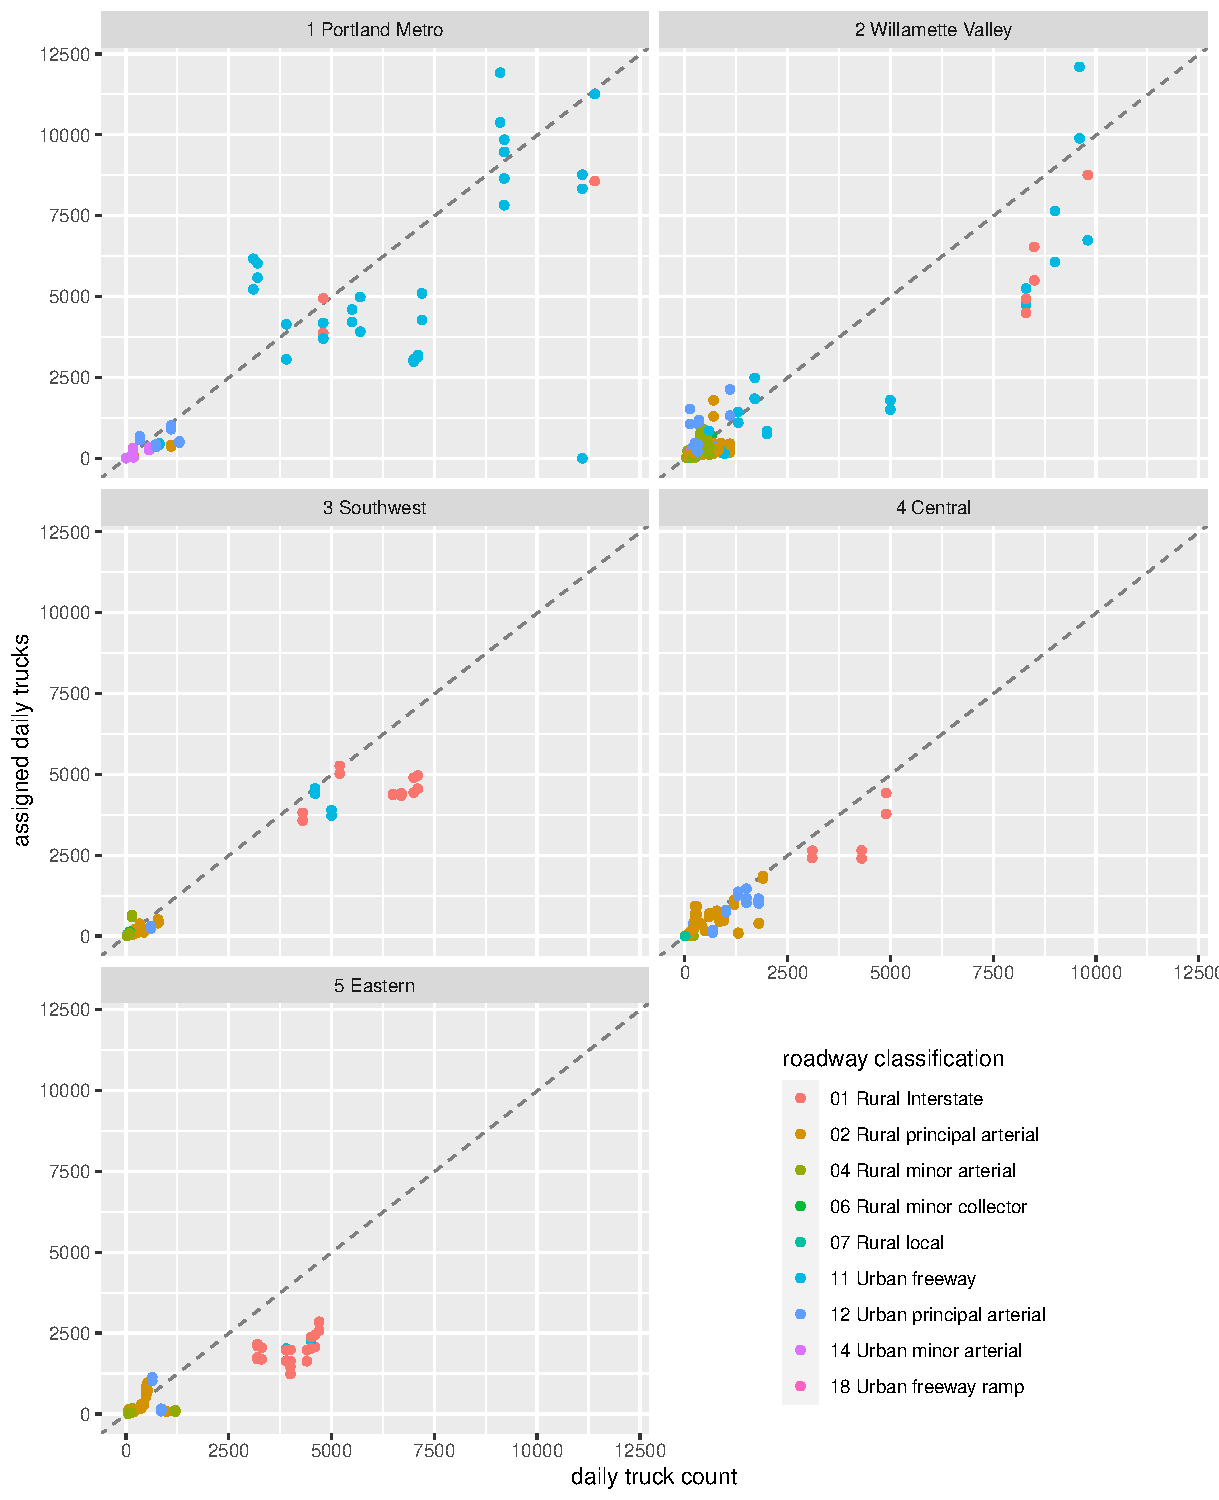
\includegraphics[width=6.5in]{figures/graph-final-validation-scatter.pdf}
\caption{Observed versus estimated truck flows at selected Oregon count locations}
\label{fig:ct-link-scattergram}
\end{figure}

Statistical measures provide a more definitive criteria for evaluating model performance, and can be compared to results obtained in similar models. The root mean squared error (RMSE) is commonly used to compare how well the model replicates observed truck counts:
\begin{equation}
RMSE = \sqrt {\sum_{i \in I} O_i - A_i \over (n - 1)}
\end{equation}

\noindent where $O_i$ and $A_i$ are the observed and assigned flows on link $i$, respectively, for the set of links $I$ that count data are available for. A percent, or normalized, RMSE statistic can then be calculated to scale the error to range of the data, similar to the coefficient of variation:
\begin{equation}
PRMSE = (RMSE \div \bar O) \times 100
\end{equation}

\noindent These statistics are typical compiled for subsets of the network, as shown in Table \ref{tab:ct-assignment-statistics}. There is no formal guidance on what constitutes an acceptable result. In urban person travel models a PRMSE target of 25 percent is often used for freeways and higher-volume arterials, while values between 50 and 75 percent are often accepted for smaller volume roadways. However, truck flows are often complex (\S\ref{sec:ct-tour-complexity}) and exhibit higher variances than auto traffic (\S\ref{sec:ct-large-variances}). Thus, higher PRMSE values are often encountered in truck models used across North America. When judged within that context the results appear quite reasonable. This is readily apparent when looking at the corresponding graph in Figure \ref{fig:ct-link-scattergram}, which reveals that the model has a tendency to under-estimate observed truck counts in the Willamette Valley and in eastern Oregon. Experiments to better tune to the model to replicate patterns in those two ODOT regions resulted in poorer fits in the remaining regions. The results shown in Figure \ref{fig:ct-link-scattergram} resulted in the best overall fit of the model to all count data. 

The results can also be compared to criteria suggested in NCHRP Report 765 \citep{cdmsmith14}. The maximum desirable error (MDE) is a function of the count volume. A variant of Figure 4-3 from their report compares the percent error at each count location to the count volume.\footnote{The absolute percent error is compared to the count for each point in Figure 4-3 of the report. That shows the extent of the error, but not its directionality. Retaining the sign of the percent error can reveal whether a systematic pattern of under or over-assignment is present. The pattern shown in Figure \ref{fig:ct-mde-comparison} is symmetrical, suggesting that is not an issue in this case.} The MDE points would all fall between the curves shown in Figure \ref{fig:ct-mde-comparison} in an ideal model. Note that the curves diverge from the x-axis (i.e.,  percent error of zero) for the smaller volumes typically associated with truck flows. An ideal outcome is rarely achieved, and models with only a few points outside of the line are considered quite robust. It is clear that the CT module achieves this criteria, with only a few points lying outside of the curves. These summaries provide confidence that the emergent behavior from the CT module replicates well the truck travel patterns within Oregon.

\begin{table}
\centering
\caption{Validation summary statistics}
\label{tab:ct-assignment-statistics}

\begin{tabular}{lrrrrrr}
\\[-5pt]
\multicolumn{7}{c}{(a) Summary by ODOT regions} \\
\hline
Region & n & Avg count & CV count & avg assigned & RMSE & PRMSE \\
\hline
1 Portland Metro & 55 & 4,163 & 0.91 & 3,444 & 2,246 & 0.54 \\
\gray 2 Willamette Valley & 114 & 1,514 & 1.75 & 1,155 & 1,072 & 0.71 \\
3 Southwest & 48 & 2,146 & 1.25 & 1,608 & 1,002 & 0.47 \\
\gray 4 Central & 68 & 1,060 & 1.09 & 773 & 574 & 0.54 \\
5 Eastern & 66 & 1,680 & 1.09 & 873 & 1,308 & 0.78 \\
\end{tabular}

\begin{tabular}{lrrrrrr}
\\[-5pt]
\multicolumn{7}{c}{(b) Summary by roadway classification} \\
\hline
Classification & n & Avg count & CV count & avg assigned & RMSE & PRMSE \\
\hline
01 Rural Interstate & 46 & 5,265 & 0.37 & 3,462 & 2,035 & 0.39 \\
\gray 02 Rural principal arterial & 122 & 526 & 0.76 & 346 & 418 & 0.79 \\
04 Rural minor arterial & 49 & 255 & 1.03 & 197 & 291 & 1.14 \\
\gray 06 Rural minor collector & 3 & 463 & 0.7 & 445 & 106 & 0.23 \\
07 Rural local & 6 & 71 & 0.68 & 22 & 71.7 & 1.01 \\
\gray 11 Urban freeway & 57 & 5,597 & 0.57 & 4,482 & 2,526 & 0.45 \\
12 Urban principal arterial & 58 & 788 & 0.67 & 669 & 491 & 0.62 \\
\gray 14 Urban minor arterial & 8 & 230 & 0.97 & 149 & 178 & 0.78 \\
18 Urban freeway ramp & 2 & 150 & 0 & 164 & 77 & 0.51 \\
\hline
\end{tabular}
\end{table}


\begin{figure}
\centering
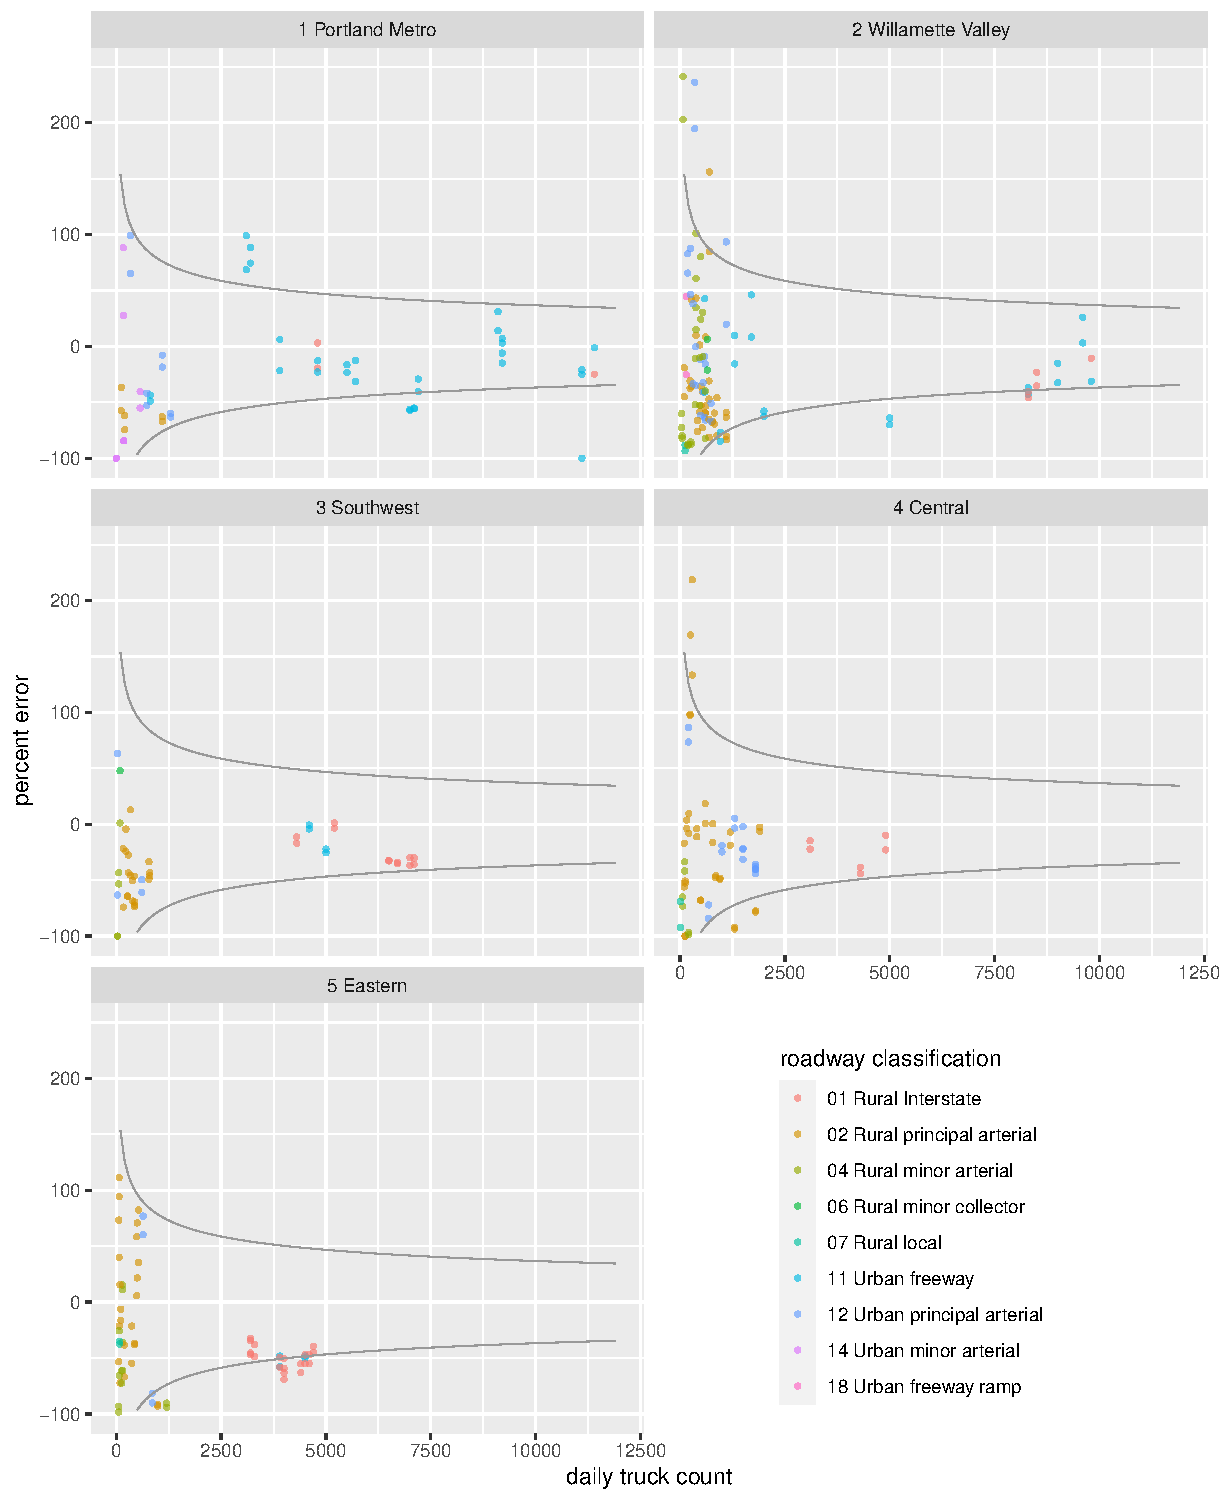
\includegraphics[width=6.5in]{figures/graph-final-validation-trumpet.pdf}
\caption{Comparison of percent error of assigned flows to truck counts}
\label{fig:ct-mde-comparison}
\end{figure}

\section{Current status}

The current CT module is a stable platform that has undergone several changes over the past several years. The local truck modeling portion has changed little since its original formulation, owing in part to a lack of Oregon data from which to improve it, the rather slow rate of innovation in urban truck modeling, and a larger focus on regional rather than local issues in SWIM2 applications. Moreover, it has continued to perform acceptably in validation over several SWIM2 development cycles and model applications. 

The long-distance modeling portion of the CT module has undergone extensive updating over the past few years. The older approach of fusing the Commodity Flow Survey with AA outputs has been replaced by a process that converts the FAF commodity flow estimates and forecasts into long-distance truck trips within, into and out of, and through Oregon. The flows are now constrained to match observed or asserted volumes at the SWIM2 external zones, eliminating the last remaining large source of large errors in CT validation. 

The collection and processing of establishment survey and truck GPS tracking data will be required to further improve the CT module. Experience elsewhere suggests that a tour-based modeling approach will continue to better leverage the limited data available and provide the flexibility for model evolution and application. Until that time continued updates to the FAF will likely improve the model fit statistics without the need to retool the underlying software.


% Copy the bibliography file directly from the treso-doc repo
\bibliography{devguide}
\end{document}
